% Trustworthy credit risk scoring: PRML course project report (Step 17).
% Build from the project root:  make report   ->  reports/report.pdf
\documentclass[conference,10pt]{IEEEtran}
\usepackage[utf8]{inputenc}
\usepackage[T1]{fontenc}
\renewcommand{\ttdefault}{lmtt}   % monospace: Courier is not installed in TinyTeX
\usepackage{amsmath,amssymb}
\usepackage{graphicx}
\usepackage{booktabs}
\usepackage{xcolor}
\usepackage[hidelinks]{hyperref}
\graphicspath{{../figures/}}

% A shaded "in simple terms" box: the idea before the details
\newcommand{\simple}[1]{\par\smallskip\noindent\colorbox{gray!13}{\parbox{\dimexpr\columnwidth-2\fboxsep\relax}{\small\textbf{In simple terms.} #1}}\par\smallskip}
\newcommand{\demourl}{\url{https://trustworthy-credit-risk-rchtsc9esc5kj5mvuq86kb.streamlit.app/}}

\begin{document}

\title{Trustworthy Credit Risk Scoring:\\Calibrated, Explained and Fair Loan Decisions\\with a Guarantee}

\author{\IEEEauthorblockN{Amartya Gawali (EP23BT010)}
\IEEEauthorblockA{PRML course project, IIT Dharwad, 2026\\
Code: \url{https://github.com/INKiE1911/trustworthy-credit-risk}\\
Live demo: \demourl}}

\maketitle

\begin{abstract}
A lender has to decide, for every applicant, whether to lend. We build a complete loan-default
system on the Home Credit Default Risk data (307,511 labelled applications in 7 linked tables)
and ask not only how accurate it is but whether each of its outputs can be trusted. A tuned
LightGBM on 240 leak-free features reaches a test ROC-AUC of \textbf{0.790} (95\% CI
0.784--0.797), exactly its cross-validation estimate, and ranks applicants significantly better
than logistic regression, a glass-box EBM and a bank-style points scorecard. Its probabilities
are already calibrated (expected calibration error 0.0018), so a break-even money rule earns
\textbf{13.9\%} more than approving everyone. A class-conditional conformal layer approves,
refers or declines with a written promise: on the untouched test split only \textbf{9.8\%} of
defaulters were auto-approved, against a promised 10\%. Every decision is explained with
TreeSHAP reason codes and an actionable ``what would change it'' answer; fairness is audited by
gender and age (reweighing cuts the gender gap in wrongly declined good customers from 4.6 to
2.0 points at equal accuracy); and drift is watched with the population stability index. The
report explains each idea from first principles, with worked examples on the real numbers.
\end{abstract}

% =========================================================================================
\section{Introduction}
\label{sec:intro}

\subsection{The problem}
When someone applies for a loan, the lender must answer one question: \emph{will this person
repay?} Two kinds of mistakes are possible:
\begin{itemize}
\item approving someone who then \emph{defaults} (does not repay): the lender loses money;
\item declining someone who \emph{would} have repaid: the lender loses a good customer, and the
person loses access to credit.
\end{itemize}
The two mistakes do not cost the same, and if the second one happens more often to some groups
of people than to others it can be unfair and, in many countries, unlawful.

Machine learning can learn from past loans which applicants tend to default. This is a
\emph{supervised classification} problem: every past application has a label (defaulted or
not), and the model learns a function from the application's data to a \emph{probability of
default}, a number between 0 and 1.

\subsection{What ``trustworthy'' means here}
A model that is merely accurate is not enough for a real lending decision. We break trust into
six questions, and each later section answers one of them:
\begin{enumerate}
\item \textbf{Does it rank applicants well?} Are risky people scored higher than safe ones
(Sec.~\ref{sec:models}, \ref{sec:test})?
\item \textbf{Are its probabilities honest?} When it says 10\%, do about 10\% of such people
default (Sec.~\ref{sec:decisions})?
\item \textbf{Can its errors be controlled?} Can we promise an upper limit on wrongly approved
defaulters and wrongly declined good customers (Sec.~\ref{sec:decisions})?
\item \textbf{Can it explain itself?} Can it say \emph{why} an applicant was declined, and what
would change the answer (Sec.~\ref{sec:xai})?
\item \textbf{Is it fair?} Does it treat men and women, young and old, similarly
(Sec.~\ref{sec:fair})?
\item \textbf{Does it keep working?} Will we notice when new applicants stop looking like the
old ones (Sec.~\ref{sec:system})?
\end{enumerate}

\subsection{How the project was run}
The work was done in 18 numbered steps on the Kaggle Home Credit Default Risk
data~\cite{homecredit2018}. Three rules were kept throughout:
(i) every number in this report comes from a notebook in the repository;
(ii) every model is compared on the same five cross-validation folds, with confidence intervals;
(iii) 20\% of the data, the \emph{test split}, was locked away and opened exactly once, at the
very end, so the final numbers are an honest estimate of performance on new applicants.

\textbf{Contributions.}
(i) A leak-free feature pipeline over 7 related tables (240 features) and a ladder of 14 models
compared with bootstrap confidence intervals and paired tests.
(ii) Two controlled experiments: class-imbalance ``fixes'' make the model worse, and SMOTE is
recognised by the trees; three tuning methods at the same budget.
(iii) Seven classical algorithms written from scratch in NumPy that match scikit-learn.
(iv) A decision layer: a calibration check, a break-even money threshold, and a conformal
approve/refer/decline rule whose error promise was verified on the test split.
(v) Explanations (TreeSHAP, a LIME check, PDP, actionable counterfactuals), a fairness audit
with three mitigations and an impossibility demonstration on the real base rates, risk personas,
and a drift monitor.
(vi) A working service (FastAPI + Streamlit, in Docker) with a public demo that uses only made-up
applicants and a stand-in model, so neither the real data nor the real model is published.

Table~\ref{tab:syllabus} maps the work to the 16 units of the course.

\begin{table*}[t]
\centering\small
\caption{Syllabus coverage: where each course unit appears in the project.}
\label{tab:syllabus}
\begin{tabular}{@{}rlp{12.6cm}@{}}
\toprule
\# & Unit & What this project does \\
\midrule
1 & Introduction & Credit scoring framed as pattern recognition with unequal error costs (Sec.~\ref{sec:intro}, \ref{sec:decisions}). \\
2 & Types of ML & Supervised (default prediction), unsupervised (segments, personas), semi-supervised as the reject-inference problem (Sec.~\ref{sec:ethics}), reinforcement learning as future work. \\
3 & Preprocessing & Data traps (365243 code, XNA), imputation, one-hot / target / WoE encoding, scaling, 7-table aggregation, feature selection inside each fold. \\
4 & Regression & Logistic regression (Newton's method from scratch); ridge vs least squares to predict \texttt{EXT\_SOURCE\_1} ($R^2=0.405$). \\
5 & Classification & Decision tree (depth curve), KNN, linear and RBF SVM, Naive Bayes; confusion matrix and all metrics. \\
6 & Clustering & K-means++, Gaussian mixture with EM and BIC, Ward hierarchical, HDBSCAN; silhouette, Davies--Bouldin, Calinski--Harabasz, adjusted Rand index. \\
7 & Dimensionality reduction & PCA and Fisher LDA from scratch; scree plot; t-SNE at three perplexities. \\
8 & Ensembles & Bagging (random forest, out-of-bag score), AdaBoost, gradient boosting (LightGBM, XGBoost, HistGB), EBM. \\
9 & Neural networks & NumPy MLP with hand-written backpropagation (gradient check $2\times10^{-7}$); PyTorch MLP with embeddings. \\
10 & Probabilistic models & MLE vs MAP (L2 = Gaussian prior), Laplace Bayesian logistic regression, Gaussian NB, EM, calibration. \\
11 & Evaluation & Stratified frozen splits, 5-fold CV, ROC/PR/KS, bootstrap CIs, paired bootstrap, McNemar, 5$\times$2cv t-test, Holm correction, learning curves. \\
12 & Tuning & Grid vs random vs Bayesian optimisation (Optuna TPE) at the same budget. \\
13 & Practical ML & Python package, 14 notebooks, 133 unit tests, continuous integration, MLflow tracking. \\
14 & Explainable AI & Gain, permutation and SHAP importance, PDP/ICE, LIME, scorecard, EBM, counterfactuals, reason codes. \\
15 & Applications & A complete credit-decision system with an API, a web app and monitoring. \\
16 & Ethics & Fairness audit, proxy test, impossibility demonstration, 3 mitigations, privacy, model card, datasheet, human review. \\
\bottomrule
\end{tabular}
\end{table*}

% =========================================================================================
\section{Background: the Key Ideas}
\label{sec:background}
This section explains, from the beginning, the measuring tools used everywhere else.

\subsection{From a probability to a decision: the confusion matrix}
The model outputs a probability of default $p$. To make a decision we pick a threshold $t$ and
decline everyone with $p \ge t$. Calling a defaulter a ``positive'', every applicant falls in one
of four boxes (Table~\ref{tab:confusion}).

\begin{table}[h]
\centering\small
\caption{The confusion matrix, with the counts of our final model on the test split at the money threshold $t = 0.1667$ (61,502 applicants).}
\label{tab:confusion}
\begin{tabular}{@{}lcc@{}}
\toprule
 & Declined ($p \ge t$) & Approved ($p < t$) \\
\midrule
Defaulted & TP $\approx$ 2,203 & FN $\approx$ 2,762 \\
Repaid & FP $\approx$ 5,481 & TN $\approx$ 51,056 \\
\bottomrule
\end{tabular}
\end{table}

From these four numbers:
the \emph{true-positive rate} (TPR, recall) $= \mathrm{TP}/(\mathrm{TP}+\mathrm{FN})$ is the share
of defaulters we catch (44.4\%); the \emph{false-positive rate} (FPR) $= \mathrm{FP}/(\mathrm{FP}+\mathrm{TN})$
is the share of good customers we wrongly decline (9.7\%); the \emph{precision}
$= \mathrm{TP}/(\mathrm{TP}+\mathrm{FP})$ is the share of declined people who really would have
defaulted; and accuracy is $(\mathrm{TP}+\mathrm{TN})/N$ (86.6\%).

\textbf{Why accuracy is misleading here.} Only 8.07\% of applicants default. A ``model'' that
approves everyone is 91.93\% accurate and catches nobody. Accuracy rewards ignoring the rare
class, so we use the measures below instead.

\subsection{Measuring a ranking: ROC curve and AUC}
Moving the threshold $t$ from 1 down to 0 traces the \emph{ROC curve}: FPR on the x-axis, TPR on
the y-axis. A useless model gives the diagonal; a perfect one goes straight up to the top-left
corner. The area under it, \emph{ROC-AUC}, is between 0.5 (random) and 1 (perfect).

\simple{ROC-AUC is the probability that the model gives a \emph{randomly chosen defaulter} a
higher risk than a \emph{randomly chosen good customer}. Our 0.790 means: pick one of each at
random, and 79\% of the time the defaulter gets the higher score.}

Related numbers: the \textbf{Gini} coefficient banks quote is $2\,\mathrm{AUC}-1$ (0.580 for us);
the \textbf{KS} statistic is the largest gap between TPR and FPR over all thresholds (0.439);
\textbf{PR-AUC} is the area under the precision--recall curve, which focuses on the rare
defaulters (random guessing gives 0.081, the default rate; we get 0.295).

\subsection{Measuring honesty: calibration}
A ranking can be perfect while the probabilities are wrong (for example if every probability
were divided by two). For money decisions we need \emph{calibrated} probabilities.

\simple{A model is calibrated if, among all applicants it gives about 10\%, about 10\% really
default; among those it gives 30\%, about 30\% default; and so on.}

Two measures: the \textbf{Brier score} is the average of $(p_i - y_i)^2$ where $y_i \in \{0,1\}$
is the true outcome (lower is better); the \textbf{expected calibration error} (ECE) sorts
applicants into probability bins and averages, weighted by bin size, the gap between the mean
predicted probability and the actual default rate in each bin. A \emph{reliability diagram}
plots one against the other; a calibrated model lies on the diagonal.

\subsection{Honest evaluation}
\textbf{Splits.} If a model is tested on data it learned from, it looks better than it is
(\emph{overfitting}). We therefore split the labelled data once: a \emph{train} split to learn
from, a \emph{validation} split to make decisions about the system (threshold, calibration,
fairness), a \emph{conformal} split reserved for the conformal layer, and a \emph{test} split
that is used once at the end.

\textbf{Cross-validation (CV).} To compare models on the train split without wasting data, it is
cut into 5 equal \emph{folds}. Each model is trained 5 times, each time on 4 folds and scored on
the fifth, so every applicant is scored exactly once by a model that never saw them
(\emph{out-of-fold} predictions).

\textbf{Leakage.} Anything learned from data, such as the median used to fill missing values,
must be learned inside each training fold only; otherwise information from the scored fold
``leaks'' in. All such steps live inside scikit-learn pipelines that are refitted per fold.

\textbf{Uncertainty: the bootstrap.} A score from one data set is itself uncertain. The
bootstrap~\cite{efron1993} resamples the scored applicants with replacement 1,000 times and
recomputes the score each time; the middle 95\% of those values is the 95\% confidence interval
(CI). To compare two models we use the \emph{paired} bootstrap: the same resamples for both, and
a CI for the \emph{difference}. If that CI does not contain 0, the difference is significant.

\textbf{Many tests at once.} If we run four tests at the 5\% level, the chance of at least one
false alarm is much larger than 5\%. The Holm correction~\cite{holm1979} multiplies the smallest
p-value by 4, the next by 3, and so on, keeping the overall false-alarm rate at 5\%.

\subsection{The winning model family: gradient-boosted trees}
A \emph{decision tree} asks a sequence of yes/no questions (``is the external score below
0.3?'') and ends in a leaf that predicts a risk. One deep tree overfits; one shallow tree is too
simple. \emph{Gradient boosting}~\cite{friedman2001} adds many shallow trees one after another;
each new tree is fitted to correct the errors the current sum of trees still makes, and its
contribution is shrunk by a small \emph{learning rate}. LightGBM~\cite{ke2017} and
XGBoost~\cite{chen2016} are fast implementations; they handle missing values and categories
natively.

\simple{Boosting is like a team of weak experts where each new expert studies only the cases
the team still gets wrong. 1,871 small trees, each adding a small correction, make the final
model.}

% =========================================================================================
\section{Related Work}
\textbf{Credit scoring.} Logistic regression on weight-of-evidence (WoE) bins, turned into a
points table, is the industry standard because it is transparent~\cite{thomas2002,siddiqi2006}.
Large benchmarks find that ensembles, especially boosting, rank applicants
better~\cite{lessmann2015}.

\textbf{Boosting on tabular data.} Gradient boosting~\cite{friedman2001,chen2016,ke2017} is the
strongest family on tabular data and still beats deep networks there~\cite{grinsztajn2022}.
Explainable boosting machines (EBM) keep the model additive and readable~\cite{nori2019}.

\textbf{Probabilities and decisions.} Platt scaling~\cite{platt1999} and isotonic
regression~\cite{zadrozny2002} recalibrate scores; boosted trees are often already close to
calibrated~\cite{niculescu2005}. With calibrated probabilities the cost-optimal decision is a
threshold set by the costs~\cite{elkan2001,bishop2006}.

\textbf{Conformal prediction} gives prediction sets with a finite-sample guarantee under
exchangeability~\cite{vovk2005,angelopoulos2021}; class-conditional (Mondrian) versions give the
guarantee for each class separately.

\textbf{Explainability.} SHAP values~\cite{lundberg2017} are exact and fast for trees
(TreeSHAP~\cite{lundberg2020}); LIME~\cite{ribeiro2016} fits local surrogate models.
Counterfactual explanations~\cite{wachter2018} should only change features a person can act
on~\cite{ustun2019}.

\textbf{Fairness.} Equal opportunity asks for equal true-positive rates across
groups~\cite{hardt2016}; here, equal approval of good customers. Calibration within groups and
equal error rates cannot both hold when base rates differ~\cite{kleinberg2017,chouldechova2017}.
Mitigations act before training (reweighing~\cite{kamiran2012}), during training
(reductions~\cite{agarwal2018}) or after training (group thresholds~\cite{hardt2016}). Model
cards~\cite{mitchell2019} and datasheets~\cite{gebru2021} document models and data.

% =========================================================================================
\section{Data}
\label{sec:data}

\subsection{Seven linked tables}
Home Credit lends to people with little or no credit history. The data has one row per
application in the main table and six history tables linked to it by the applicant id
\texttt{SK\_ID\_CURR} (Table~\ref{tab:tables}). The label \texttt{TARGET} is 1 if the client had
payment difficulties on the loan.

\begin{table}[h]
\centering\small
\caption{The seven tables (rows after conversion to Parquet).}
\label{tab:tables}
\footnotesize\setlength{\tabcolsep}{3pt}
\begin{tabular}{@{}lrl@{}}
\toprule
Table & Rows & One row is \ldots \\
\midrule
application (train) & 307,511 & an application, with the label \\
application (test) & 48,744 & an application, no label \\
bureau & 1,716,428 & a loan at another lender \\
bureau\_balance & 27,299,925 & a month of such a loan \\
previous\_application & 1,670,214 & an earlier application here \\
installments\_payments & 13,605,401 & an instalment payment \\
POS\_CASH\_balance & 10,001,358 & a month of a POS/cash loan \\
credit\_card\_balance & 3,840,312 & a month of a credit card \\
\bottomrule
\end{tabular}
\end{table}

The model needs exactly one row per applicant, so every history table is summarised per
applicant (Sec.~\ref{sec:features}). Coverage differs a lot: 94.8\% of applicants have
instalment records, 85.7\% have bureau records, but only 30.0\% have monthly bureau statuses and
28.3\% have credit cards.

\subsection{What the exploratory analysis found}
\textbf{Imbalance.} 24,825 of 307,511 applicants defaulted (8.07\%).

\textbf{Traps.}
\begin{itemize}
\item 55,374 rows (18.0\%) have \texttt{DAYS\_EMPLOYED} = 365243 (that is, 1,000 years in the
future). It is a code for ``no employment record'', mostly pensioners, who default at 5.40\% vs
8.66\% for everyone else. We turned it into ``missing'' plus a flag, because the flag itself is
informative. The same code hides in five date columns of the previous applications.
\item Four rows have gender ``XNA''; they were dropped.
\item Income is extremely skewed: median 147,150, maximum 117 million; we use its logarithm.
\item 41 of 122 columns are more than half empty (mostly building descriptions), and 64 pairs of
numeric columns correlate above 0.9 (the building \texttt{\_AVG/\_MODE/\_MEDI} triples).
\end{itemize}
Two bugs were caught only because results were checked against the raw data: counting split
payments row by row claimed 67\% of instalments were underpaid (0\% once payments are combined
per instalment), and the 365243 code had quietly emptied two previous-loan features.

\textbf{Strongest single signals.} Three ``external scores'' (normalised scores from outside
credit bureaus) have the largest rank correlations with default ($-0.166$, $-0.151$,
$-0.147$; a higher score means lower risk).

\textbf{Groups.} Men default at 10.14\% vs 7.00\% for women; applicants under 30 at 11.44\% vs
4.92\% at 60 and over. These different \emph{base rates} matter in the fairness section.

\textbf{Drift preview.} The Kaggle test file is a different mix: 0.9\% revolving loans vs 9.52\%
in the training file.

\subsection{Splits}
The labelled rows were split once, stratified by the label so each split has the same 8.07\%
default rate (Table~\ref{tab:splits}). The split file refuses to be overwritten.

\begin{table}[h]
\centering\small
\caption{Frozen splits of the labelled applications.}
\label{tab:splits}
\setlength{\tabcolsep}{4pt}
\begin{tabular}{@{}lrrl@{}}
\toprule
Split & Rows & Share & Used for \\
\midrule
train & 184,503 & 60\% & learning, 5-fold CV \\
validation & 30,751 & 10\% & calibration, money rule, fairness \\
conformal & 30,751 & 10\% & conformal cut-offs only \\
test & 61,502 & 20\% & final evaluation, once \\
\bottomrule
\end{tabular}
\end{table}

The 48,744 unlabelled Kaggle test applications are never used for evaluation, only for the demo
and as a real example of drift.

% =========================================================================================
\section{Features}
\label{sec:features}
\simple{A model cannot read 27 million monthly rows. For each applicant we summarise each
history table into a few numbers, such as ``how many earlier loans were refused'' or ``how many
months were paid late in the last year''.}

\textbf{Per table.} Each history table is aggregated per applicant with its own key: counts,
sums, means, maxima, recent-window counts (for example late months in the last year), and
late-payment rates. Applicants with no history get count features of 0 and a
\texttt{HAS\_HISTORY} flag; averages stay missing. Payments are first combined per instalment,
and bureau monthly statuses per bureau loan, before summarising.

\textbf{Engineered ratios.} The most useful features combine raw columns: the mean, minimum and
maximum of the three external scores; annuity divided by loan amount (how fast the loan is
repaid); loan amount above the price of the goods; bureau debt divided by income; total
repayment burden; current loan size compared with past loans.

\textbf{Result.} 241 columns: application 121, bureau 31, bureau balance 9, previous
applications 32, instalments 22, POS/cash 12, credit cards 14. Gender is kept only for the
fairness audit, so the model uses \textbf{240 features}.

\textbf{One code path.} The same function builds the application features for training and for
the app, so a ``what-if'' change in the app is processed exactly as in training.

% =========================================================================================
\section{Models}
\label{sec:models}

\subsection{The model ladder}
Fourteen models were trained on the same five folds, from the simplest to the strongest
(Table~\ref{tab:ladder}). In one line each:
\begin{itemize}
\item \textbf{Dummy}: predicts the average rate for everyone (the floor, AUC 0.5).
\item \textbf{Naive Bayes}: Bayes' rule assuming features are independent given the class.
\item \textbf{Decision tree}: one tree of yes/no questions.
\item \textbf{KNN}: the risk of the most similar past applicants.
\item \textbf{Linear / RBF SVM}: a separating line, or a curved boundary via a kernel.
\item \textbf{Logistic regression}: a weighted sum of features passed through the sigmoid
$1/(1+e^{-z})$.
\item \textbf{WoE scorecard}: logistic regression on binned features, turned into a points
table, as banks use.
\item \textbf{Random forest} (bagging): many deep trees on random samples, averaged.
\item \textbf{AdaBoost}: tiny trees, each focusing on the cases the previous ones got wrong.
\item \textbf{Gradient boosting} (HistGB, XGBoost, LightGBM): Sec.~\ref{sec:background}.
\item \textbf{EBM}: a boosted model that is a \emph{sum of one curve per feature}, so it can be
read like a scorecard.
\end{itemize}

\begin{table}[t]
\centering\small
\caption{Five-fold CV ROC-AUC on the train split (184,503 applicants, 240 features).}
\label{tab:ladder}
\begin{tabular}{@{}lcc@{}}
\toprule
Model & ROC-AUC & 95\% CI \\
\midrule
\textbf{Tuned LightGBM (final)} & \textbf{0.790} & 0.787--0.793 \\
LightGBM, default settings & 0.787 & \\
XGBoost & 0.785 & \\
HistGradientBoosting & 0.783 & \\
EBM (glass box) & 0.776 & \\
Logistic regression & 0.776 & 0.772--0.779 \\
PyTorch MLP (embeddings) & 0.772 & 0.768--0.775 \\
Linear SVM & 0.772 & 0.768--0.775 \\
RBF SVM (Nystroem) & 0.764 & 0.760--0.768 \\
Random forest & 0.763 & 0.759--0.766 \\
AdaBoost & 0.757 & 0.753--0.760 \\
WoE scorecard (30 features) & 0.755 & 0.751--0.758 \\
KNN & 0.746 & 0.742--0.750 \\
Decision tree (depth 8) & 0.725 & 0.721--0.730 \\
Naive Bayes on 30 PCA comp. & 0.708 & 0.704--0.713 \\
\midrule
LightGBM, main table only & 0.761 & 0.758--0.765 \\
Dummy & 0.500 & \\
\bottomrule
\end{tabular}
\end{table}

\textbf{What the ladder shows.}
\begin{itemize}
\item The three gradient-boosting libraries are within 0.003 of each other: the \emph{method}
matters, not the library.
\item Logistic regression is only 0.010--0.014 behind, because the engineered ratios already
capture much of the non-linear signal.
\item The decision tree shows overfitting clearly: it is best at depth 6 (held-out 0.725); at
depth 20 it scores 0.905 on its own training data but only 0.519 on new data.
\item Naive Bayes is poor on raw features (0.543). With 240 correlated features it counts the
same evidence many times and becomes so overconfident that 82.3\% of applicants get a
probability of exactly 1.0, which ROC-AUC cannot rank (ties). Ranked by its log-odds it reaches
0.664, and on 30 uncorrelated PCA components 0.708.
\item The random forest's built-in out-of-bag score (0.763) equals its CV score (0.763).
\end{itemize}

\subsection{Does the loan history help? (ablation)}
\simple{An ablation removes or adds one ingredient at a time to see how much each one is
worth.}

Starting from the main table alone (0.761), we added one history table at a time
(Fig.~\ref{fig:ablation}). The bureau adds the most (+0.0097), then previous applications
(+0.0055), instalments (+0.0053), POS/cash (+0.0021) and credit cards (+0.0022): +0.025 in total,
with non-overlapping confidence intervals. Each table adds less than the one before, because
later tables partly repeat what earlier ones show.

\begin{figure}[t]
\centering
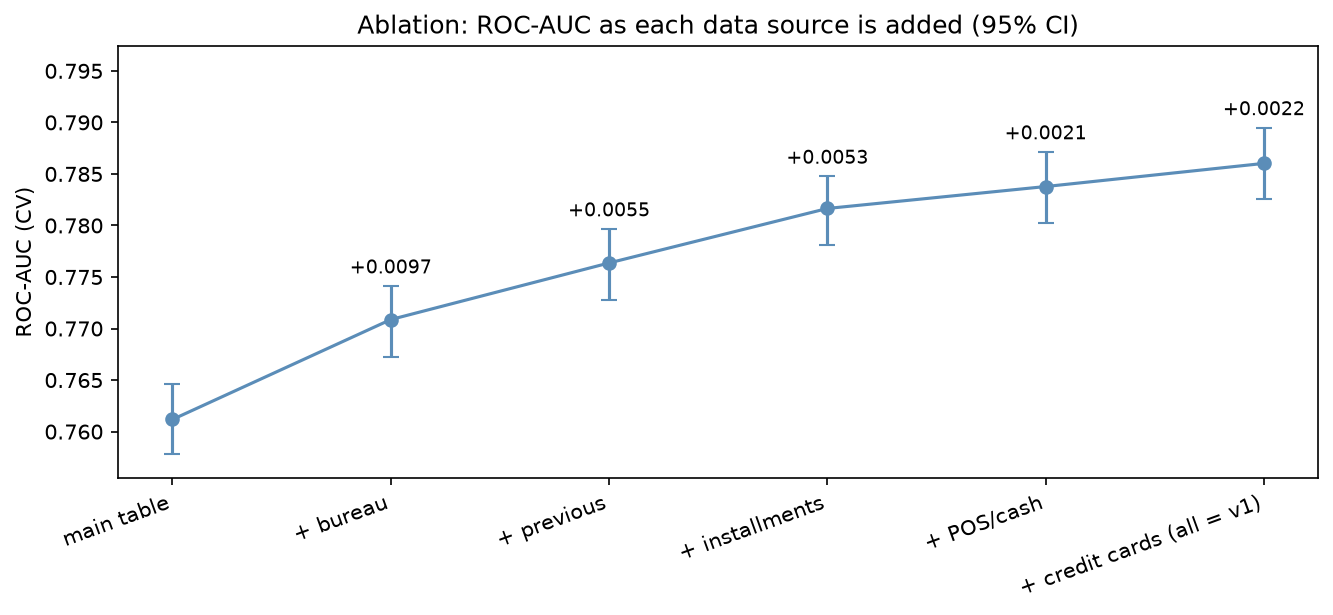
\includegraphics[width=\columnwidth]{fig12_ablation.png}
\caption{Ablation: CV ROC-AUC as each history table is added (95\% CI).}
\label{fig:ablation}
\end{figure}

\subsection{Experiment 1: should we ``fix'' the class imbalance?}
With only 8\% defaulters, a common recommendation is to rebalance the data: give defaulters a
higher weight, throw away some good customers (\emph{undersampling}), or create synthetic
defaulters with \textbf{SMOTE}~\cite{chawla2002}, which draws a new point on the line between a
defaulter and one of its nearest defaulter neighbours.

\textbf{Result.} Every ``fix'' made the ranking significantly \emph{worse} (class weights
$-0.0017$, undersampling $-0.0038$, SMOTE $-0.0039$; Table~\ref{tab:imbalance} in the appendix).
Weights and undersampling also destroyed calibration: the average predicted probability rose to
0.335 and 0.270, against a true rate of 0.081.

\textbf{The SMOTE surprise.} SMOTE also trained on 1 defaulter per 2 others, yet its average
probability stayed honest (0.084). The reason: a point between two real applicants often has a
value no real person has, such as 1.4 children. Every synthetic row had at least one such
in-between value, and a model could separate synthetic from real defaulters perfectly (ROC-AUC
1.000). The trees learned to recognise fake applicants and gave real ones roughly their real
rate. \textbf{Decision:} train on the natural 8\% rate.

\subsection{Experiment 2: tuning}
LightGBM has settings (\emph{hyperparameters}) such as the number of leaves per tree or the
learning rate. We compared three ways of searching them, each with the same budget of 27 trials,
scored on fold 1 with early stopping:
\begin{itemize}
\item \textbf{grid search} tries every combination on a fixed grid;
\item \textbf{random search} samples combinations at random~\cite{bergstra2012};
\item \textbf{TPE} (Optuna~\cite{akiba2019,bergstra2011}) builds a probability model of which
settings score well and samples where good results are likely.
\end{itemize}
Best scores: grid 0.7927, random 0.7928, TPE 0.7942 (default settings 0.7894). The differences
between methods are smaller than the noise on one fold. In full 5-fold CV the tuned model scores
0.7899 vs 0.7870, a significant +0.0029, but smaller than the +0.0048 seen on the fold used for
tuning: choosing the best of many trials on one fold makes that fold look too good (the
``winner's curse''). The final model has 1,871 trees of 17 leaves, at least 426 applicants per
leaf, and a learning rate of 0.022: many small, heavily regularised trees.

\subsection{Neural networks}
A PyTorch MLP with learned embeddings for categories (two hidden layers of 256 and 128 units,
batch normalisation, 30\% dropout, early stopping) reached 0.772, 0.018 behind LightGBM. A 50/50
blend of the two was \emph{worse} than LightGBM alone ($-0.0040$): their predictions correlate
at 0.887, so the network mostly makes the same mistakes while being weaker. This matches the
finding that trees still beat deep learning on tabular data~\cite{grinsztajn2022}.

\subsection{Algorithms from scratch}
To show the mathematics is understood, seven algorithms were written in NumPy and checked against
scikit-learn on the same data (Table~\ref{tab:scratch} in the appendix):
\begin{itemize}
\item \textbf{Logistic regression by Newton's method.} Minimising the log-loss plus an L2
penalty is the same as finding the most probable weights under a Gaussian prior (\emph{MAP}).
Newton's method uses the curvature and converges in about 10 steps. The \textbf{Laplace} version
approximates the posterior by a Gaussian around that optimum, giving each applicant an
uncertainty. Finding: uncertainty is not risk; the 10\% most uncertain applicants default at
6.4\% vs 8.5\%.
\item \textbf{Gaussian Naive Bayes}, \textbf{PCA} via the singular value decomposition, and
\textbf{Fisher LDA} (the direction that best separates the classes).
\item \textbf{K-means++} (careful random starts, then alternate ``assign to nearest centre'' and
``move centre to the mean'') and a \textbf{Gaussian mixture fitted by EM}, which never lowered
the likelihood in 50 rounds.
\item An \textbf{MLP with hand-written backpropagation}, whose gradients match numerical
derivatives to $2\times10^{-7}$.
\end{itemize}

% =========================================================================================
\section{Final Evaluation on the Test Split}
\label{sec:test}
\simple{The test split is like the final exam paper: kept sealed while studying, opened once.
Everything that could be chosen was chosen before it was opened.}

\textbf{What was fixed in advance.} The models: the final LightGBM, its reweighed version
(Sec.~\ref{sec:fair}), and logistic regression, the EBM and the scorecard refitted once on the
whole train split. The tests: the final model against each other model. The decision rules: the
money threshold and the conformal cut-offs, unchanged.

\textbf{Two significance tests.}
\begin{itemize}
\item The \textbf{paired bootstrap} on ROC-AUC asks: does the final model \emph{rank} better?
\item The \textbf{McNemar test}~\cite{mcnemar1947} asks: does it make better \emph{decisions}
at the threshold? It looks only at applicants where exactly one of the two models is right. If
the models were equally good, each such case would be a coin flip; a lopsided count is
evidence of a real difference.
\end{itemize}
Each family of four tests is Holm-corrected. Separately, \textbf{Dietterich's 5$\times$2cv
t-test}~\cite{dietterich1998} (five repetitions of a 2-fold split) compares LightGBM with
logistic regression; it retrains models, so it uses the train split only.

\textbf{Results} (Table~\ref{tab:test}, Fig.~\ref{fig:test}).
\begin{itemize}
\item Every model scores within 0.005 of its CV estimate: neither model choice nor tuning
overfitted the folds. The final model: ROC-AUC 0.790, KS 0.439, PR-AUC 0.295, Brier 0.0653,
ECE 0.0018.
\item LightGBM \emph{ranks} significantly better than all three reference models (all $p<0.001$
after Holm). The 5$\times$2cv test agrees for logistic regression ($+0.011$, $t=5.38$, $p=0.003$,
positive in all 10 halves).
\item On \emph{decisions} the gap almost vanishes: 86.6\% correct vs 86.2--86.4\%. McNemar is
significant only against logistic regression ($p=0.0005$); against the EBM and the scorecard
$p=0.066$. Most of the ranking advantage lies away from the one threshold that matters.
\item The \textbf{price of transparency} is 0.009 ROC-AUC for the EBM, with indistinguishable
decision accuracy.
\end{itemize}

\begin{table}[t]
\centering\small
\caption{Frozen test results (61,502 applicants, 8.07\% default). $\Delta$AUC is the final model's advantage (paired bootstrap).}
\label{tab:test}
\footnotesize\setlength{\tabcolsep}{2.5pt}
\begin{tabular}{@{}lcccc@{}}
\toprule
Model & ROC-AUC [95\% CI] & PR-AUC & Brier & $\Delta$AUC \\
\midrule
\textbf{LightGBM (final)} & \textbf{0.790}\,{\scriptsize[0.784, 0.797]} & 0.295 & 0.0653 & -- \\
LightGBM, reweighed & 0.790\,{\scriptsize[0.784, 0.797]} & 0.294 & 0.0653 & $+0.000$ \\
EBM (glass box) & 0.781\,{\scriptsize[0.774, 0.788]} & 0.273 & 0.0663 & $+0.009^\ast$ \\
Logistic regression & 0.778\,{\scriptsize[0.771, 0.785]} & 0.272 & 0.0664 & $+0.013^\ast$ \\
WoE scorecard & 0.757\,{\scriptsize[0.751, 0.765]} & 0.239 & 0.0679 & $+0.033^\ast$ \\
\bottomrule
\multicolumn{5}{@{}l}{\scriptsize $^\ast$ significant after Holm correction. Final model: KS 0.439, Gini 0.580, ECE 0.0018.}
\end{tabular}
\end{table}

\begin{figure*}[t]
\centering
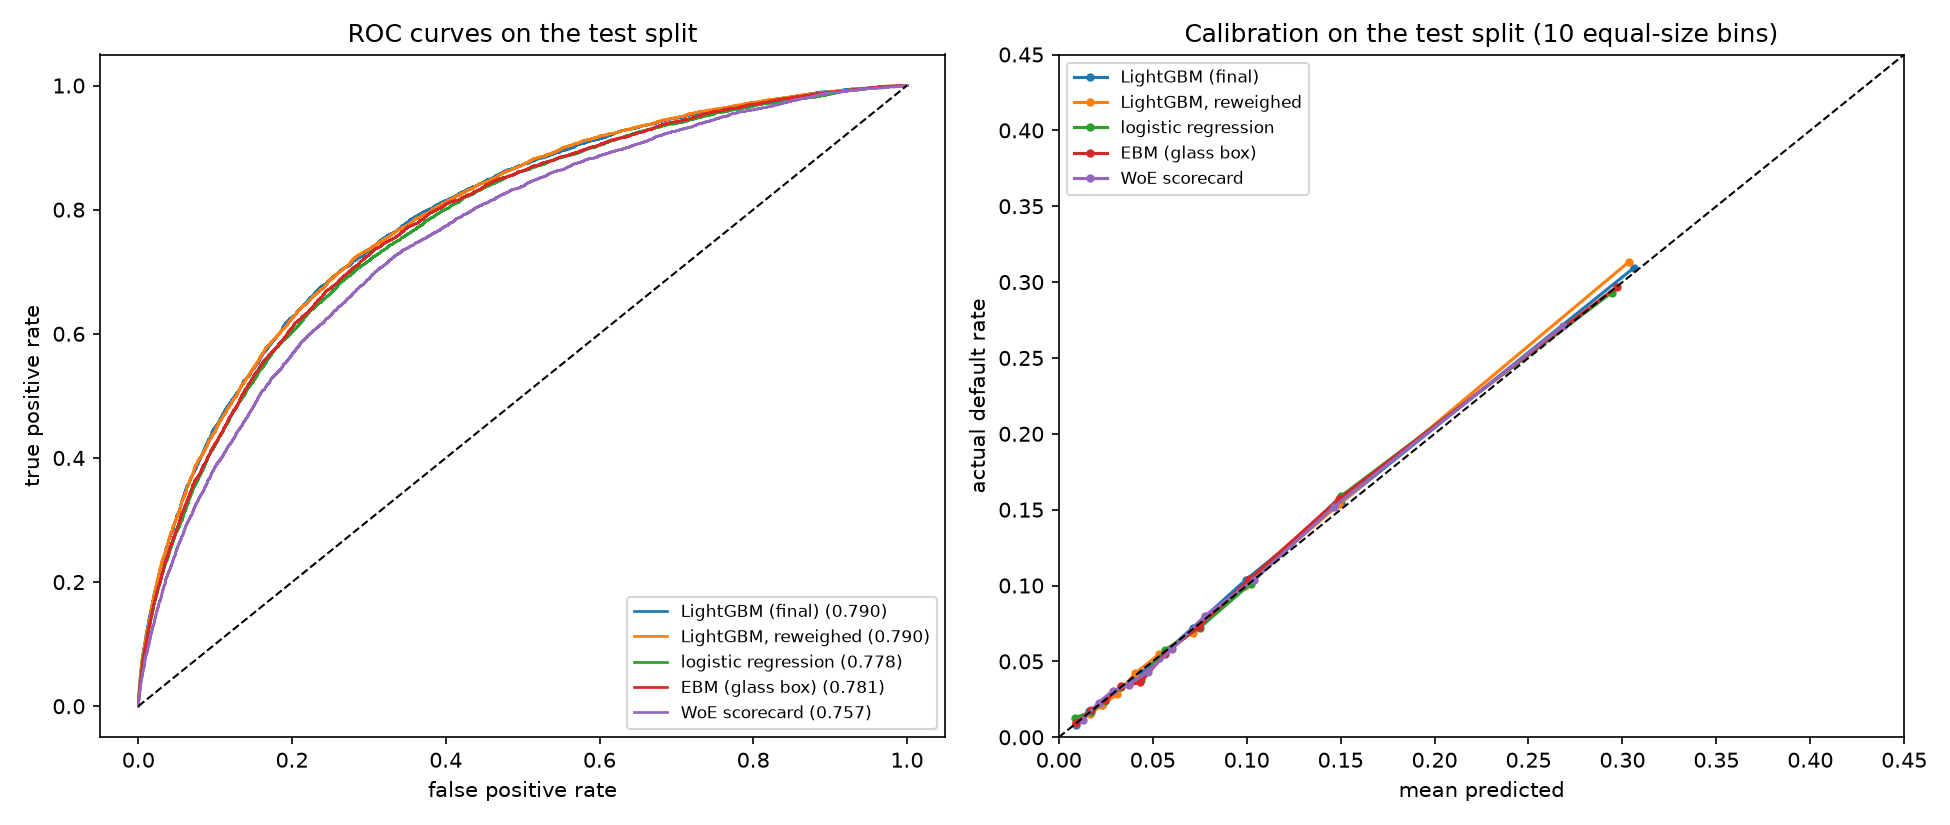
\includegraphics[width=0.8\textwidth]{fig38_test_roc_calibration.png}
\caption{Test split: ROC curves (left) and calibration in ten equal-size bins (right) for the five frozen models. All five lie on the diagonal of the calibration plot.}
\label{fig:test}
\end{figure*}

\textbf{Learning curves: would more data help?} We trained on 2\% to 100\% of four folds and
scored on the fifth (Fig.~\ref{fig:learning}). Logistic regression's training and held-out
curves have met at a low level: it is limited by its simple form (\emph{high bias}), so more
data barely helps (0.776 $\to$ 0.778 from half to all). LightGBM's training score is still far
above its held-out score (\emph{variance}), and its held-out score is still rising (0.784 $\to$
0.794): more data would help the boosted model, not the linear one.

\begin{figure}[t]
\centering
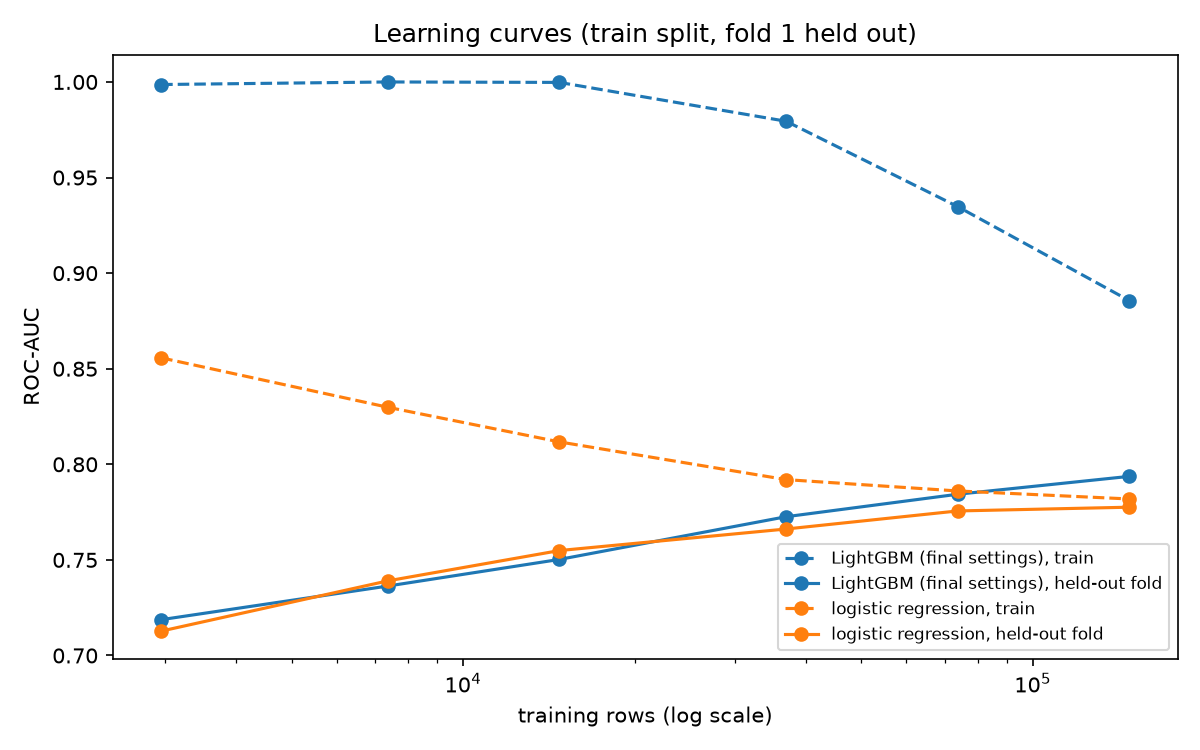
\includegraphics[width=\columnwidth]{fig37_learning_curves.png}
\caption{Learning curves (train split, fold 1 held out).}
\label{fig:learning}
\end{figure}

% =========================================================================================
\section{From Probability to Decision}
\label{sec:decisions}

\subsection{Are the probabilities honest? (calibration check)}
On the validation split the raw model was already calibrated: mean predicted 8.03\% vs 8.07\%
actual, Brier 0.06529, ECE 0.0024. We still tried two standard fixes, fitted with five-fold
cross-fitting inside the validation split so no applicant is scored by a fix that saw them:
\textbf{Platt scaling}~\cite{platt1999} fits a logistic curve to the scores, and
\textbf{isotonic regression}~\cite{zadrozny2002} fits a step function that only goes up. A fix
was kept only if its Brier improvement had a 95\% CI entirely below 0. Platt changed the Brier
score by $+0.000005$ (CI $-0.000016$ to $+0.000027$), and isotonic lowered ROC-AUC (its steps
create ties). \textbf{Decision: no calibrator.} Boosted trees with a log-loss objective are often
already calibrated~\cite{niculescu2005}, and avoiding the imbalance ``fixes'' kept it that way.
On test: 7.99\% predicted vs 8.07\% actual.

One caveat matters later: the model is calibrated \emph{overall} but not \emph{within gender}
(men 9.3\% predicted vs 10.4\% actual; women 7.4\% vs 6.9\%).

\subsection{The money rule}
\simple{Lend if the expected gain is positive.}

Suppose approving a loan of size $A$ earns a margin $m$ (say 10\%) if it is repaid, and loses a
share LGD (``loss given default'', say 50\%) if it is not. With default probability $p$, the
expected profit is
\begin{equation}
\mathbb{E}[\text{profit}] = (1-p)\,m\,A - p\,\mathrm{LGD}\,A ,
\end{equation}
which is positive exactly when
\begin{equation}
p < t^\ast = \frac{m}{m + \mathrm{LGD}} = \frac{0.10}{0.10 + 0.50} = 0.1667 .
\end{equation}

\textbf{Worked example.} A loan of 500,000 earns 50,000 if repaid and loses 250,000 if not. At
$p = 0.10$ the expected profit is $0.9 \times 50{,}000 - 0.1 \times 250{,}000 = +20{,}000$:
approve. At $p = 0.20$ it is $0.8 \times 50{,}000 - 0.2 \times 250{,}000 = -10{,}000$: decline.
The rule only works if $p$ is a real probability, which is why calibration was checked first.

\textbf{Result.} On validation the rule approves 87.4\%, declines 44.5\% of defaulters but only
9.8\% of good customers, and earns 1,144M vs 1,011M for approving everyone (+13.1\%). Searching
for the best threshold on validation finds 0.185, which earns only 0.3\% more
(Fig.~\ref{fig:profit}): decision theory gets the threshold right without any search. On test the
rule earns +13.9\%. The threshold depends on the assumed margin and loss: across plausible values
the approval rate ranges from 54\% to 99\%.

\begin{figure}[t]
\centering
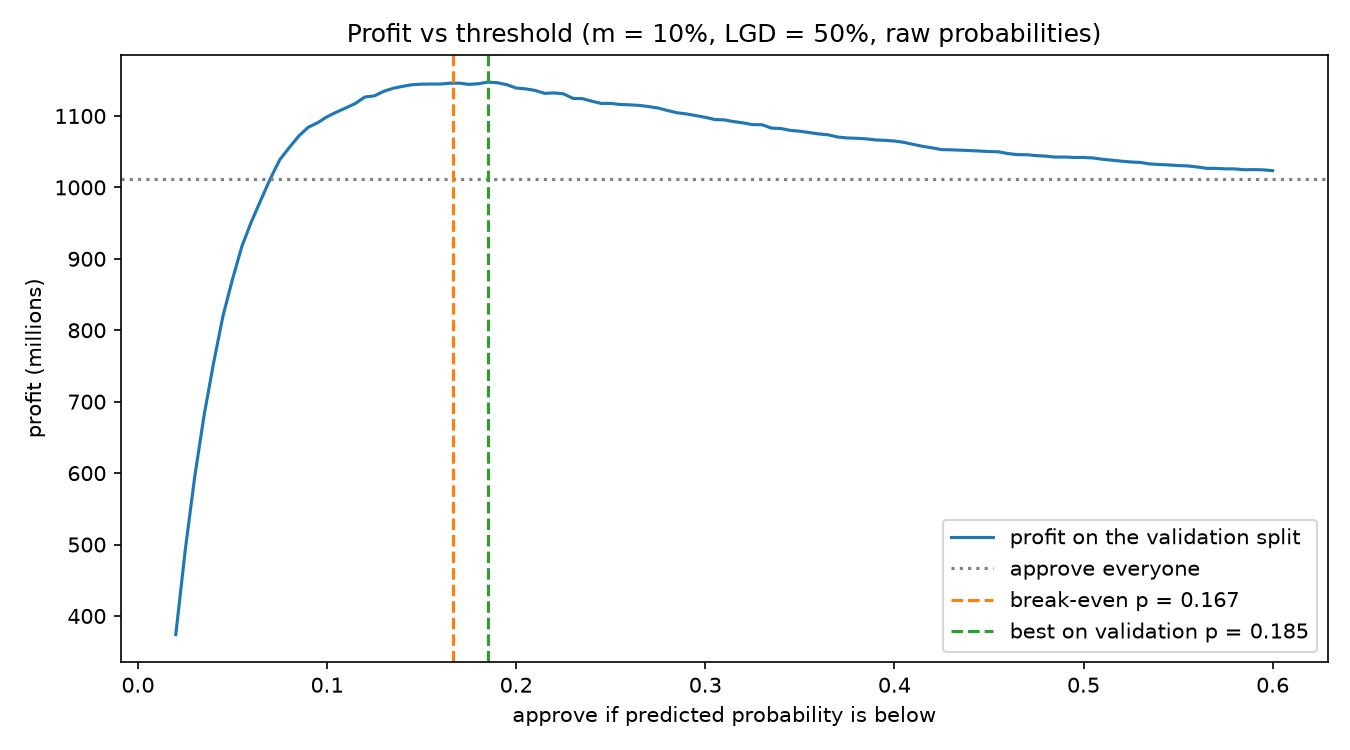
\includegraphics[width=\columnwidth]{fig21_profit_vs_threshold.png}
\caption{Validation profit vs the approval threshold. The break-even threshold (0.167) is within 0.3\% of the best one.}
\label{fig:profit}
\end{figure}

\subsection{A guarantee instead of a guess: the conformal layer}
The money rule always gives an answer, even when the model is unsure. We want a rule that
\emph{promises} limits on both mistakes and sends unclear cases to a person.

\simple{For each applicant we build a \emph{set} of answers the model cannot rule out: \{repay\},
\{default\}, or both. If only ``repay'' is left we approve; if only ``default'' is left we
decline; if both are left the model is unsure and a person decides. The cut-offs are set on
held-out data so that at most 10\% of real defaulters end up approved and at most 10\% of good
customers end up declined.}

\textbf{How it works.} Each possible answer gets a \emph{non-conformity score}: how strange that
answer would be. For ``repay'' the score is $p$ (a repayer with a high $p$ is strange); for
``default'' it is $1-p$. On the \emph{conformal} split (30,751 applicants never used for
anything else) we look at each class separately. Among the $n$ applicants who really repaid, the
cut-off $q_{\text{repay}}$ is the $\lceil (n+1)(1-\alpha)\rceil$-th smallest score, so that about
$1-\alpha$ of repayers score below it; $q_{\text{default}}$ is computed the same way among
defaulters. A new applicant's set contains ``repay'' if $p \le q_{\text{repay}}$ and ``default''
if $1-p \le q_{\text{default}}$. We use $\alpha = 10\%$.

\textbf{The cut-offs we got.} $q_{\text{repay}} = 0.1655$ and $q_{\text{default}} = 0.9645$,
which gives a simple rule: \textbf{approve if $p < 0.0355$, decline if $p > 0.1655$, refer in
between.}

\textbf{Worked example} (three real demo applicants):
\begin{itemize}
\item $p = 0.019$: ``repay'' is in the set ($0.019 \le 0.1655$), ``default'' is not
($1 - 0.019 = 0.981 > 0.9645$). Only ``repay'': \textbf{approve}.
\item $p = 0.070$: both conditions hold. Both answers possible: \textbf{refer}.
\item $p = 0.227$: ``repay'' is out ($0.227 > 0.1655$), ``default'' is in. \textbf{Decline}.
\end{itemize}

\textbf{The guarantee.} If new applicants are \emph{exchangeable} with the conformal split
(roughly: drawn from the same population), the share of defaulters whose set wrongly excludes
``default'' is at most about $\alpha$, and the same for repayers~\cite{vovk2005,angelopoulos2021}.
It needs no assumption about the model being right.

\textbf{Does it hold?} Over 100 random half-splits of the conformal split, coverage averaged
0.901 for repayers and 0.899 for defaulters. On the untouched test split it was 0.902 for both,
so \textbf{9.8\%} of defaulters were auto-approved and 9.8\% of good customers auto-declined,
as promised.

\textbf{The price.} Certainty costs automation: on test 40.5\% are approved, \textbf{46.9\%
referred} and 12.6\% declined. Fig.~\ref{fig:alpha} shows the trade-off: a smaller $\alpha$ (a
stricter promise) sends more people to the refer zone.

\textbf{Why one cut-off per class.} With a single cut-off for everyone the promise holds only
\emph{on average}, and the 92\% majority of repayers dominates it: it would have auto-approved
82\% of defaulters. Note also that the decline line (0.1655) almost equals the money threshold
(0.1667).

\begin{figure*}[t]
\centering
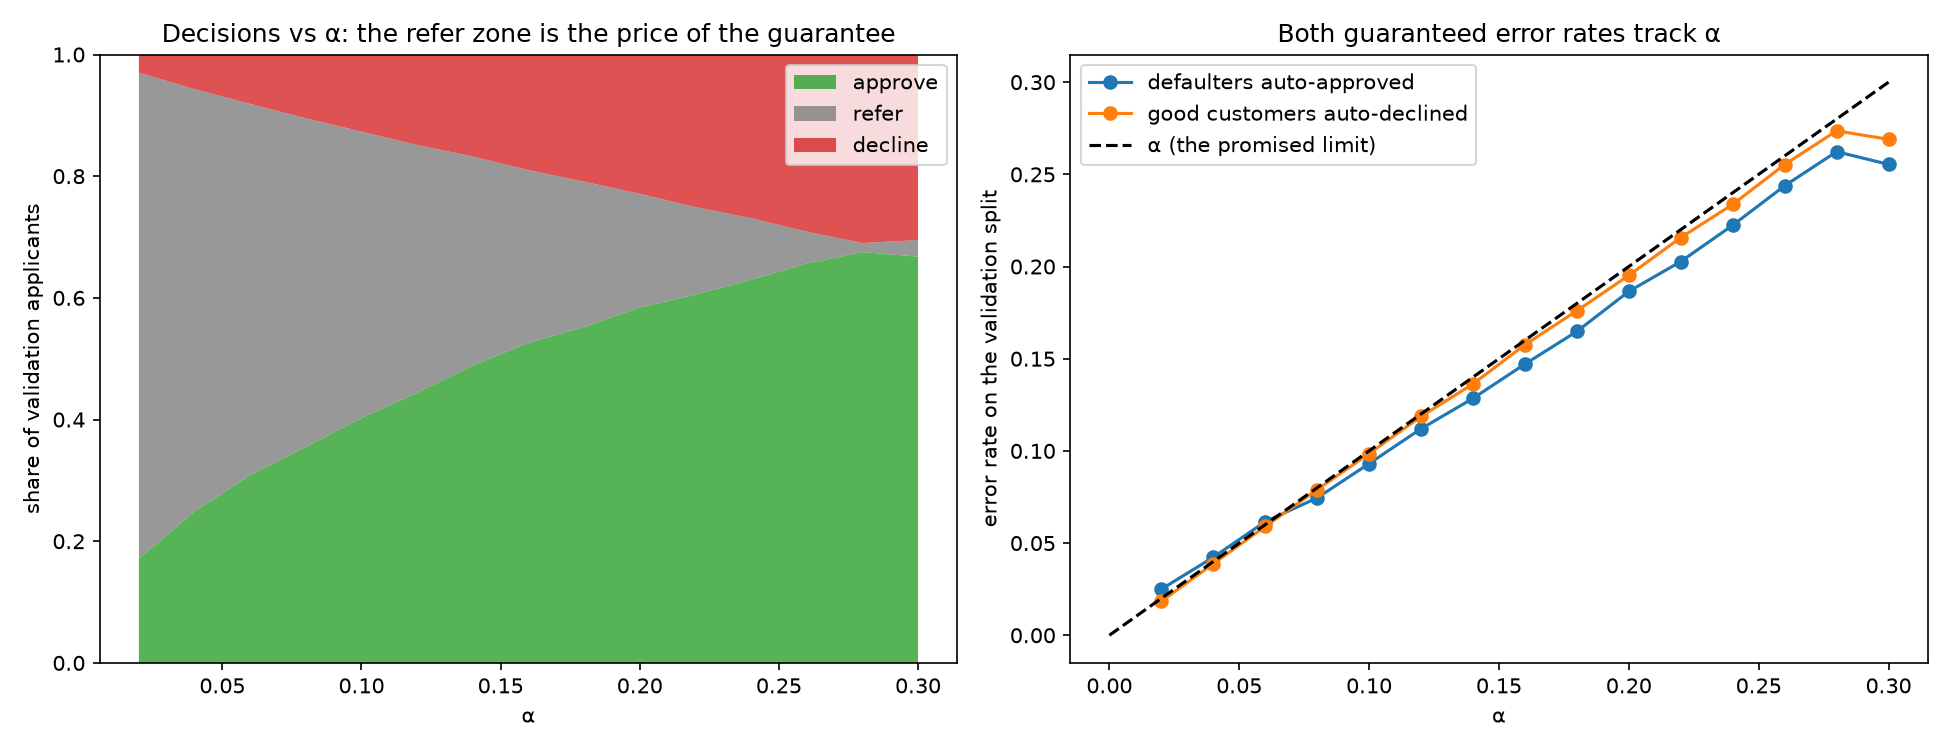
\includegraphics[width=0.78\textwidth]{fig24_decisions_vs_alpha.png}
\caption{Conformal layer on validation: decision shares (left) and the two guaranteed error rates (right) as $\alpha$ varies. Both error rates track the promised $\alpha$.}
\label{fig:alpha}
\end{figure*}

% =========================================================================================
\section{Explanations}
\label{sec:xai}

\subsection{SHAP: splitting a prediction into reasons}
\simple{Start from the risk of a typical applicant. Each feature of this applicant then pushes
the risk up or down. The pushes add up exactly to this applicant's score. The biggest upward
pushes are the reasons for a decline.}

SHAP values~\cite{lundberg2017} come from cooperative game theory: each feature gets its fair
share of the difference between this prediction and the average prediction, averaged over all
orders in which features could be added. For tree models TreeSHAP computes them exactly and
fast~\cite{lundberg2020}; LightGBM provides them directly (in log-odds units).

\textbf{Worked example.} The declined applicant from Sec.~\ref{sec:decisions} ($p = 0.227$; a
typical applicant gets 0.050) has these top upward pushes, turned into \emph{reason codes}:
\begin{itemize}
\item ``External credit scores (lowest) is 0.031, which raised the estimated risk.''
\item ``External credit scores (average) is 0.271, \ldots''
\item ``Previous applications: refused share is 0.500, \ldots''
\item ``Previous applications: total cost mean is 0.538, \ldots''
\end{itemize}
Lenders must give declined customers their main reasons (``adverse action notices'' in the
US); the app shows exactly these sentences.

\subsection{Which features matter overall?}
Three views of global importance were compared:
\textbf{gain} (how much each feature improved the trees during training),
\textbf{permutation} (how much held-out ROC-AUC drops when that feature's values are shuffled)
and \textbf{mean $|$SHAP$|$}. All three put the average external score first, and the top five
by SHAP are the average, highest and lowest external score, annuity $\div$ loan amount and
employer type. Gain and SHAP rankings agree closely (rank correlation 0.945), but permutation
and SHAP only at 0.42: when two features carry the same information, shuffling one barely hurts,
so permutation spreads the credit. 85 of the 240 features have negative permutation importance,
candidates for a simpler model.

Summing $|$SHAP$|$ per source table (Fig.~\ref{fig:shap}), the six history tables carry
\textbf{53.3\%} of the model's evidence, matching the ablation.

\begin{figure}[t]
\centering
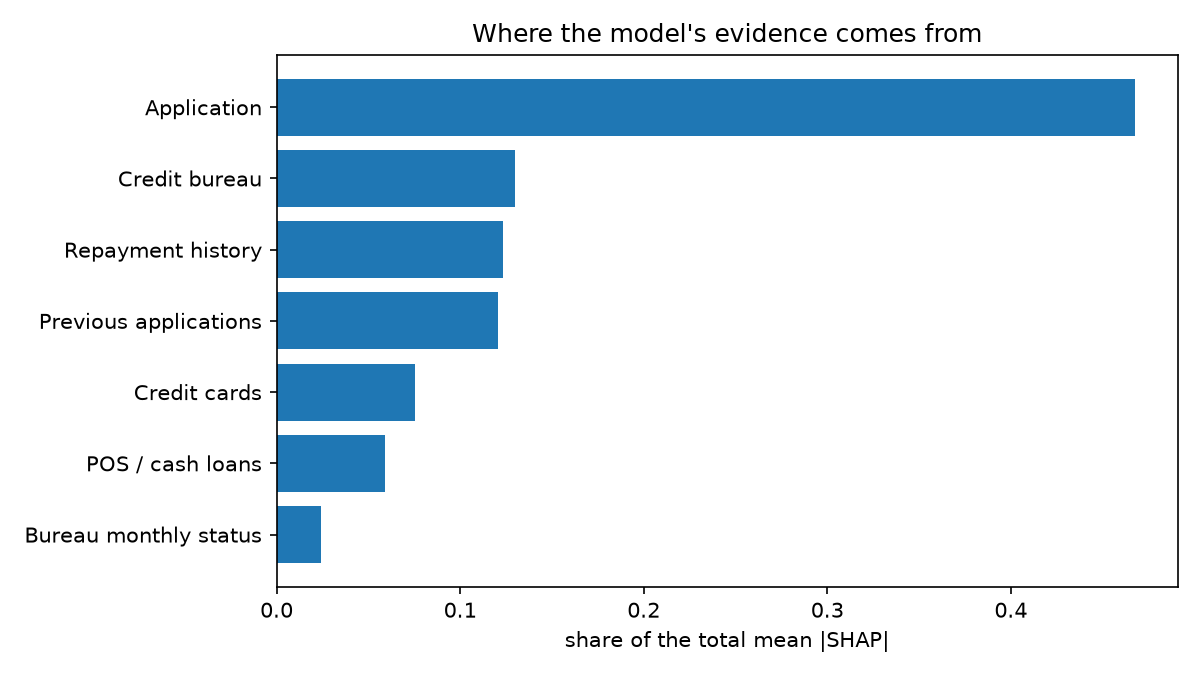
\includegraphics[width=0.92\columnwidth]{fig26_shap_by_table.png}
\caption{Share of the total mean $|$SHAP$|$ per source table.}
\label{fig:shap}
\end{figure}

\textbf{Partial dependence (PDP).} Averaging predictions while one feature is varied shows its
average effect: risk falls from about 9\% to 5\% as the average external score rises; annuity
$\div$ loan amount jumps at particular loan terms; age looks flat on its own because its signal
is shared with correlated features. A flat PDP does not mean ``no effect''.

\subsection{Is LIME a good substitute?}
LIME~\cite{ribeiro2016} explains one prediction by fitting a simple linear model to the model's
outputs on random perturbations around the applicant. Its top five reasons shared on average
2.1, 3.2 and 4.1 features with SHAP's top five for an approved, a referred and a declined
example, and changed between random seeds (Jaccard similarity 0.62--0.74). The clearer the case,
the more stable LIME is. Since TreeSHAP is exact and deterministic for this model, the app uses
SHAP.

\subsection{What would change the decision? (counterfactuals)}
\simple{Instead of ``you were declined because \ldots'', tell the applicant ``if you borrowed
X\% less, you would not be declined''.}

A counterfactual explanation~\cite{wachter2018} is the smallest change that flips the decision.
It is only useful if it changes things a person can act on~\cite{ustun2019}, so we search only
two options: a \emph{smaller loan} (loan and annuity together, in 5\% steps) and a \emph{higher
income} (10\% steps, up to 4$\times$). Age, gender and the external scores are never changed.
Every candidate goes through the real feature code, so all ratios are rebuilt.

\textbf{Results.} The declined example leaves the decline zone only when the loan is cut to 25\%
of the requested amount ($p$: 0.227 $\to$ 0.162); no income up to 4$\times$ is enough. Over all
112 declined demo applicants, \textbf{borrowing less} moves 77.7\% out of the decline zone
(median: 35\% less), while a higher income works for only 20.5\% (median $\times$1.7). For this
model the size of the loan relative to the repayment matters far more than income.

\subsection{The price of transparency}
If a regulator demanded a fully readable model: the WoE scorecard costs 0.031 ROC-AUC (CV), the
EBM only 0.010 (0.009 on test, with the same decision accuracy as LightGBM). The EBM would be the
choice.

% =========================================================================================
\section{Fairness}
\label{sec:fair}

\subsection{Definitions}
We compare groups (gender: F/M; age bands: $<$30, 30--45, 45--60, 60+) at the money rule. For
each group $g$:
\begin{itemize}
\item \textbf{approval rate};
\item \textbf{good customers declined} = FPR$_g$, the share of people who would have repaid but
were declined; the harm of a wrong rejection;
\item \textbf{defaulters declined} = TPR$_g$.
\end{itemize}
Fairness measures compare groups:
\begin{itemize}
\item \textbf{demographic parity difference}: the gap in approval rates;
\item \textbf{equal opportunity gap}~\cite{hardt2016}: the gap in good customers declined;
\textbf{our main measure}, because it protects the people a wrong rejection harms;
\item \textbf{equalized odds difference}: the larger of the FPR and TPR gaps;
\item \textbf{disparate impact ratio}: lowest approval rate $\div$ highest; the US ``80\%
rule'' flags values below 0.8.
\end{itemize}

\subsection{Audit}
Table~\ref{tab:audit} gives the validation audit (test values repeat these within about
1.5 points).

\begin{table}[t]
\centering\small
\caption{Fairness audit on validation at the money rule (percent).}
\label{tab:audit}
\setlength{\tabcolsep}{3pt}
\begin{tabular}{@{}lcccc@{}}
\toprule
Group & Default rate & Predicted & Approved & Good declined \\
\midrule
Women & 6.9 & 7.4 & 89.4 & 8.3 \\
Men & 10.4 & 9.3 & 83.7 & 12.6 \\
\midrule
Under 30 & 11.7 & 11.5 & 77.8 & 18.0 \\
30--45 & 9.2 & 8.9 & 85.2 & 11.5 \\
45--60 & 6.5 & 6.7 & 91.2 & 6.7 \\
60+ & 4.5 & 4.7 & 96.3 & 3.1 \\
\bottomrule
\end{tabular}
\end{table}

\begin{itemize}
\item \textbf{Gender:} good men are declined at 12.6\% vs 8.3\% for good women, an equal
opportunity gap of \textbf{4.3 points} against men; disparate impact 0.94.
\item \textbf{Age:} larger gaps: 18.0\% of good customers under 30 are declined vs 3.1\% at 60+;
disparate impact 0.81 on validation and \textbf{0.796 on test}, just under the 80\% line.
\item \textbf{The conformal promise holds per class, not per group:} 23\% of defaulters aged 60+
are auto-approved (target 10\%), and 18\% of good customers under 30 are auto-declined.
\end{itemize}

\subsection{Proxy test: does leaving gender out hide it?}
Gender is not a model input. But a LightGBM trained to predict gender from the other 240
features reaches ROC-AUC \textbf{0.911}, mainly through occupation, employer type and car
ownership. Deleting a column does not delete the information. The risk score itself, however,
carries little gender (0.568 when used to predict it), so the gap comes mostly from real
differences in default rates.

\subsection{Why perfect fairness is impossible here}
For any decision rule and any group, Chouldechova~\cite{chouldechova2017} showed that
\begin{equation}
\mathrm{FPR} = \frac{b}{1-b} \cdot \frac{1-\mathrm{PPV}}{\mathrm{PPV}} \cdot (1-\mathrm{FNR}),
\end{equation}
where $b$ is the group's default rate, PPV the precision of the declines and FNR the share of
defaulters missed. With our numbers it reproduces both groups' FPRs exactly (0.0833 and
0.1263). Now suppose women had the same PPV (0.306) and the same FNR (0.521) as men. With
women's default rate $b = 0.0687$ the identity forces their FPR to 0.080, against men's 0.126.

\simple{When two groups default at different rates, a rule cannot be equally precise
\emph{and} make equal mistakes for both. One kind of fairness has to give way; choosing which is
a policy decision, not a technical one~\cite{kleinberg2017}.}

\subsection{Three mitigations}
\begin{enumerate}
\item \textbf{Reweighing (before training)}~\cite{kamiran2012}: give each (group, label) cell
the weight $P(g)\,P(y)/P(g,y)$, so that in the weighted data gender and default look
independent, then retrain. Gender is needed only for training.
\item \textbf{ExponentiatedGradient (during training)}~\cite{agarwal2018}: Fairlearn trains a
mixture of models that minimises the money cost subject to an FPR gap of at most 0.01. Its
decisions are randomised (a mix of models).
\item \textbf{Group thresholds (after training)}~\cite{hardt2016}: one threshold per gender,
the most profitable pair whose gap is within a limit. Fairlearn's \texttt{ThresholdOptimizer} was
not used because it maximises accuracy, which at 8\% defaulters means approving almost
everyone.
\end{enumerate}

\begin{table}[t]
\centering\small
\caption{Gender mitigations on validation: gap in good customers declined (points) and profit relative to the final model (1,144.2M).}
\label{tab:fair}
\setlength{\tabcolsep}{4pt}
\begin{tabular}{@{}lccc@{}}
\toprule
Method & Gap & Profit & Uses gender \\
\midrule
Final model & 4.3 & -- & no \\
Reweighing (retrained) & 1.7 & $-1.2$M & no \\
ExponentiatedGradient & 1.7 & $-13.1$M & no \\
Group thresholds, gap $\le$ 1 pt & 0.8 & $-1.3$M & yes \\
Group thresholds, gap $\le$ 0.25 pt & 0.1 & $-3.6$M & yes \\
Group thresholds, no limit & 9.4 & $+1.5$M & yes \\
\bottomrule
\end{tabular}
\end{table}

\begin{figure}[t]
\centering
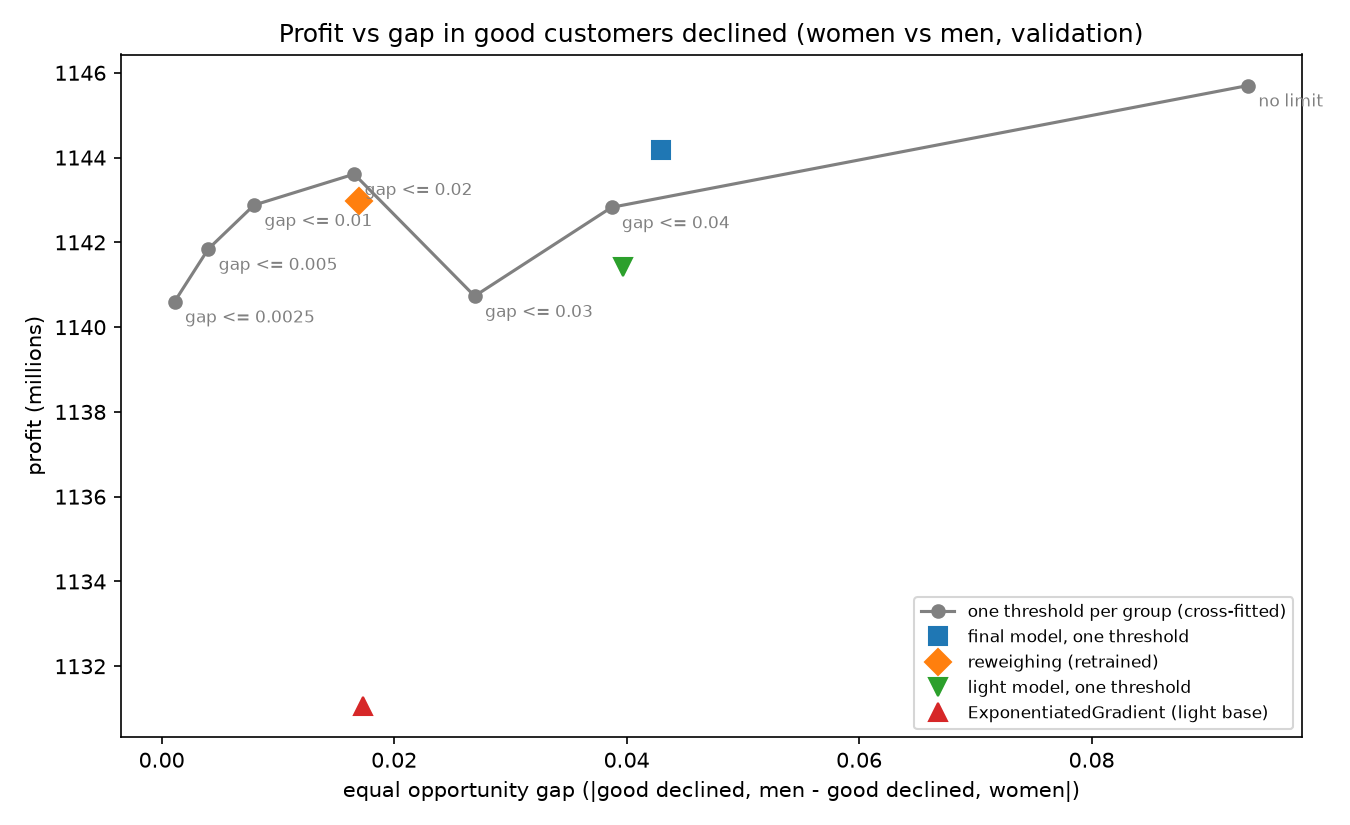
\includegraphics[width=\columnwidth]{fig32_fairness_tradeoff.png}
\caption{Profit vs the gender gap in good customers declined (validation). Differences of a few million are within noise.}
\label{fig:fair}
\end{figure}

\textbf{Results} (Table~\ref{tab:fair}, Fig.~\ref{fig:fair}). Reweighing closes 60\% of the gap
for 0.1\% of profit. ExponentiatedGradient reaches the same gap for 1.1\% of profit and gives
randomised decisions: two identical applicants could get different answers. Group thresholds
can close the gap fully, but they need gender \emph{when deciding}, which many credit laws
forbid. Strikingly, thresholds chosen for profit alone \emph{double} the gap: profit pushes away
from fairness.

\textbf{Choice and its cost.} We chose reweighing. On test it kept the same ROC-AUC (difference
0.0001, $p=0.86$) and decision accuracy, and cut the gap from 4.6 to 2.0 points for 0.55\% of
profit. The cost is the impossibility result in practice: calibration within gender got worse
(men 8.7\% predicted vs 10.2\% actual). Because the conformal cut-offs were fitted and checked on
test only for the original model, the app keeps that model, and the reweighed one is documented
as a tested alternative.

% =========================================================================================
\section{Unsupervised Learning}
\label{sec:unsup}
\simple{Without using the labels, are there natural groups of applicants, and do those groups
differ in risk?}

\textbf{Clustering} groups similar applicants. On 7 standardised key features (log income, log
loan, log annuity, family size, age, years employed, mean external score) of 20,000 train
applicants we compared four methods: \textbf{K-means} (choose $k$ by the elbow and the
\emph{silhouette}, which measures how much closer each point is to its own cluster than to the
next one, from $-1$ to 1), a \textbf{Gaussian mixture} (choose the number of components by BIC,
which rewards fit and penalises complexity), \textbf{Ward hierarchical clustering} (repeatedly
merge the two closest groups; a dendrogram shows the merges) and \textbf{HDBSCAN}~\cite{campello2013}
(clusters are dense regions; sparse points are labelled noise).

\textbf{Results.}
\begin{itemize}
\item The applicants form \textbf{one blob}: the best silhouette is only 0.19 ($k=2$, which
simply splits large loans from small ones). Ward agrees only partly (ARI 0.52); HDBSCAN finds
four pockets and calls 20\% noise.
\item \textbf{BIC can be fooled:} it prefers 9 Gaussian components, but 8 of them have zero
variance in family size: they sit on whole numbers (point masses), whose likelihood can grow
without limit. The silhouette (0.025) shows these clusters are not real.
\item \textbf{Clusters are not risk:} using a cluster's default rate as a score gives ROC-AUC
0.50--0.55 for every method, against 0.79 for the model.
\item \textbf{Maps:} the 43 numeric building columns need only 8 PCA components for 90\% of
their variance (they repeat each other); one Fisher LDA direction ranks risk at 0.714; t-SNE
shows defaulters spread everywhere, with no separate island.
\end{itemize}

\textbf{Risk personas.} Clustering the 3,897 validation applicants in the decline zone by their
\emph{SHAP vectors} groups people who are risky \emph{for the same reasons}~\cite{lundberg2020}
(Fig.~\ref{fig:personas}): ``low external scores'' (1,637 applicants, 31.0\% default),
``maxed-out credit card'' (652, 30.1\%) and ``borderline, mixed reasons'' (1,608, 25.4\%). The
structure is soft (silhouette 0.099) but tells a reviewer what to look at.

\begin{figure*}[t]
\centering
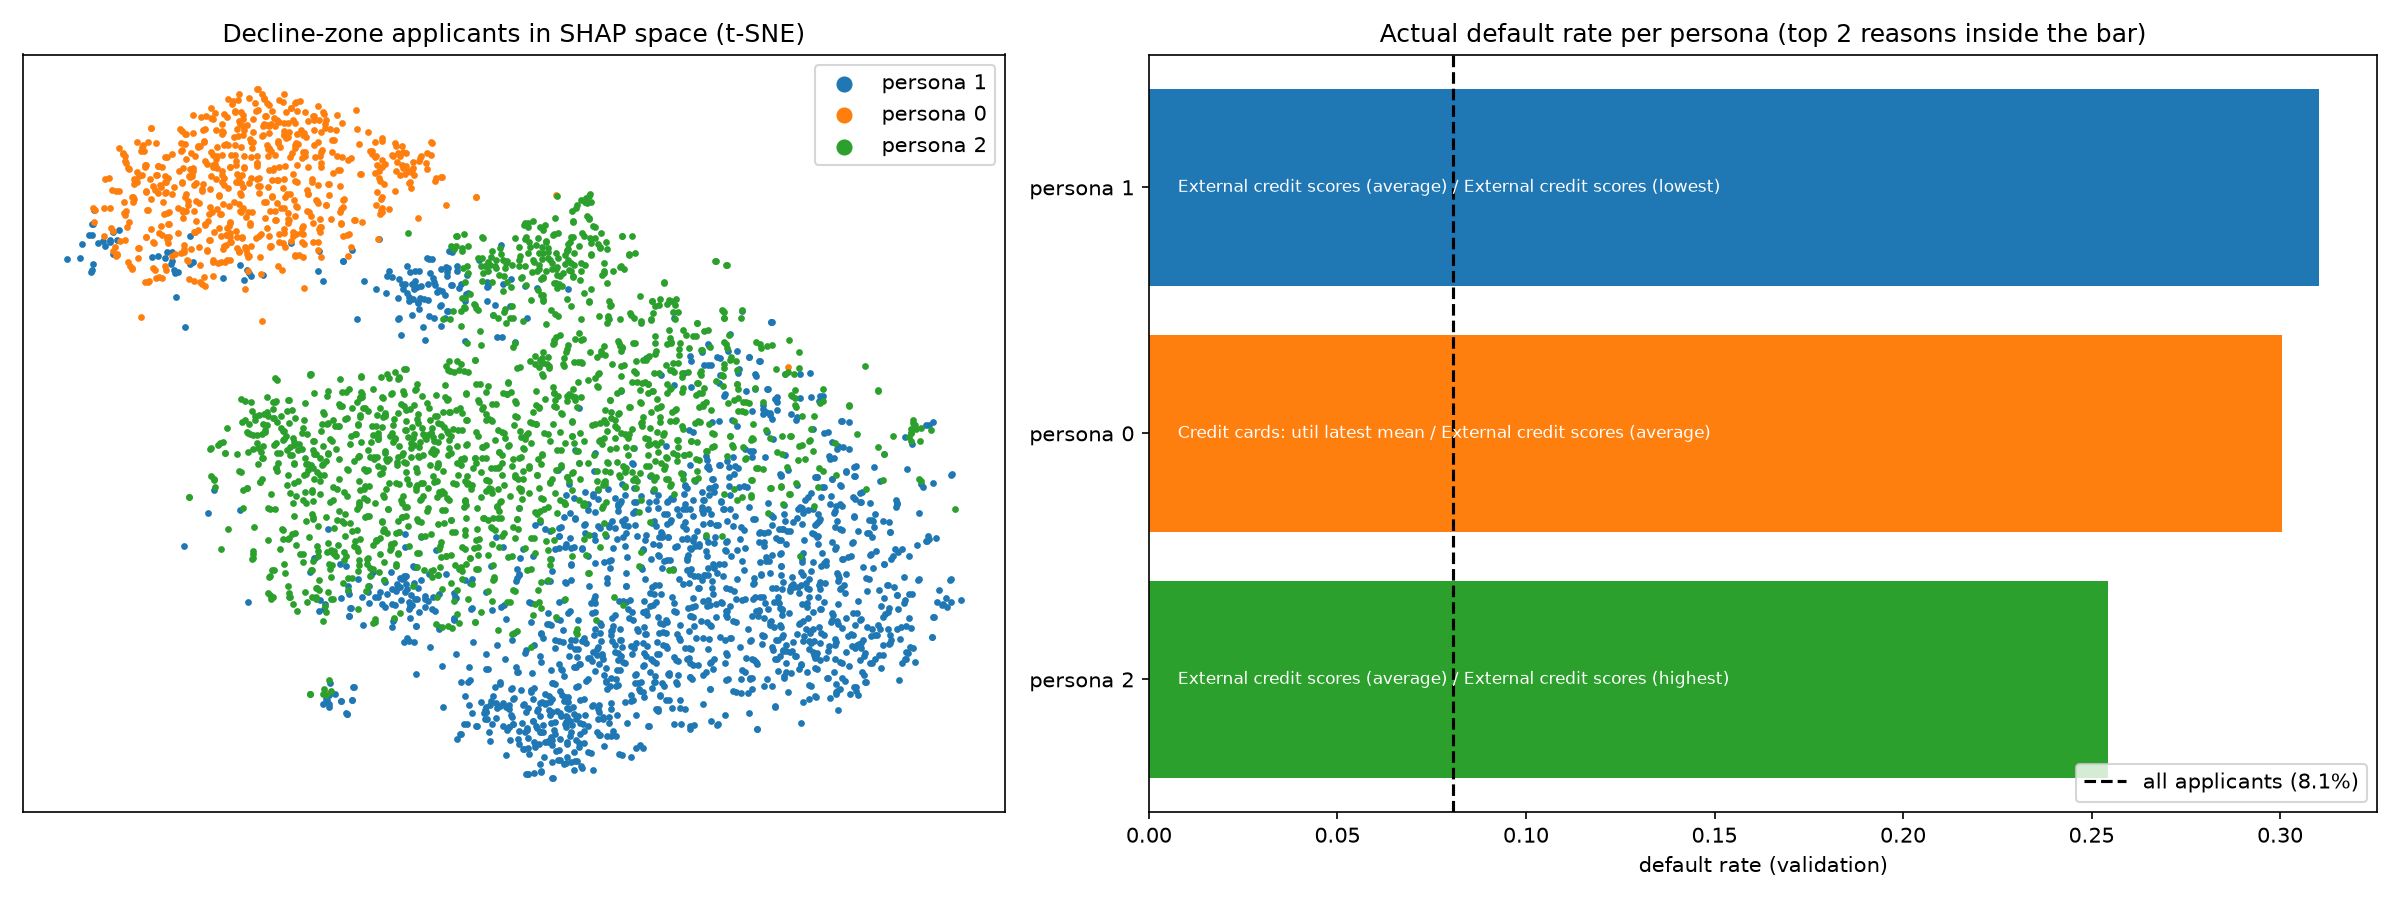
\includegraphics[width=0.8\textwidth]{fig36_risk_personas.png}
\caption{Risk personas: decline-zone applicants clustered by their SHAP values (t-SNE map, left) and each persona's actual default rate (right). Persona 1 = low external scores, persona 0 = maxed-out credit card, persona 2 = borderline.}
\label{fig:personas}
\end{figure*}

% =========================================================================================
\section{The System}
\label{sec:system}

\subsection{Architecture}
Fig.~\ref{fig:system} shows the whole pipeline. At run time a \emph{scoring service} loads the
frozen model and a small decision file (the money threshold and the conformal cut-offs). For an
applicant and up to eight ``what-if'' changes (income, loan amount, annuity, age, years employed,
three external scores) it rebuilds the features with the training code, predicts, decides, and
explains with TreeSHAP.

\begin{figure}[t]
\centering
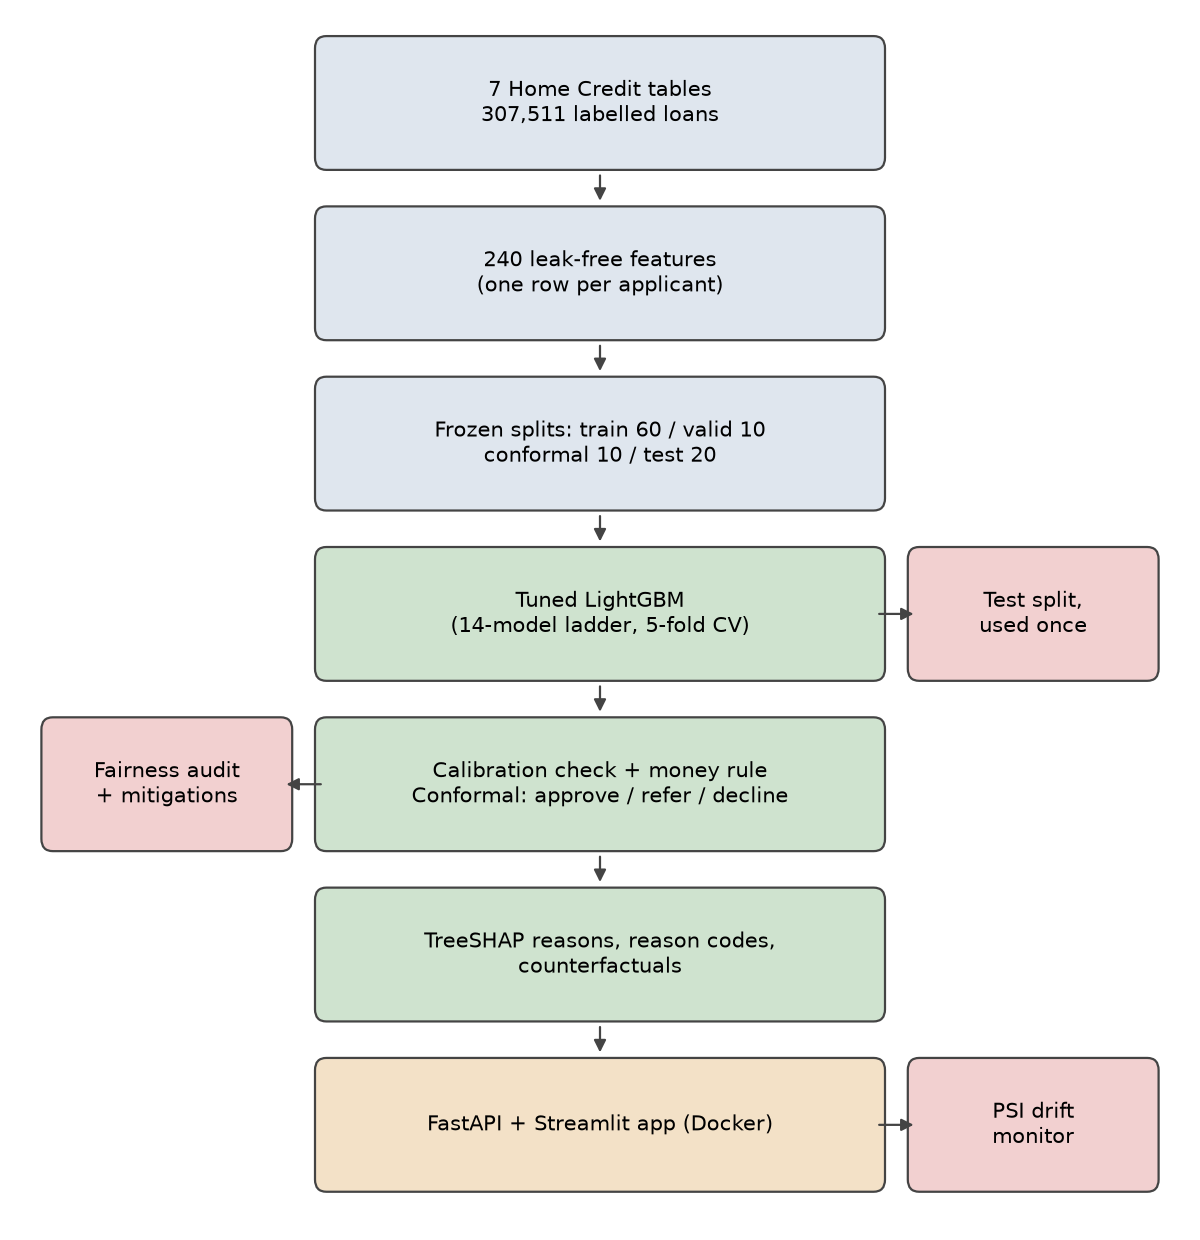
\includegraphics[width=0.9\columnwidth]{fig40_system.png}
\caption{System architecture.}
\label{fig:system}
\end{figure}

\textbf{API.} FastAPI exposes the service; Pydantic validates every input (for example,
external scores must be between 0 and 1, and years employed cannot exceed age minus 14). A call
looks like:
\begin{verbatim}
POST /score
{"applicant_id": 101383,
 "changes": {"income": 250000}}
\end{verbatim}
and returns the probability, the decision (with the money rule's suggestion), the reason codes
and the top reasons both ways. \texttt{GET /applicants/\{id\}/counterfactuals} returns the
smallest change that reaches the next better decision.

\textbf{App.} A Streamlit page with three tabs: \emph{Score + why} (probability and a reasons
chart), \emph{Decision} (approve/refer/decline with an explanation and the reason codes) and
\emph{What-if} (sliders, and a button that searches for the smallest change).

\textbf{Public demo without publishing data.} The competition rules forbid sharing the data,
and we chose not to publish the real model. The public demo (link on the title page) therefore uses 300
\emph{made-up} applicants generated with every real column, and a \emph{stand-in} model trained
only on made-up applicants, clearly labelled as such. It shows how the system works; the real
model's results are the ones in this report. The service runs in one Docker image; 133 unit
tests run on synthetic data in GitHub Actions on every push.

\subsection{Monitoring drift with PSI}
\simple{The guarantees above assume new applicants look like the old ones. The population
stability index (PSI) checks this without waiting for outcomes, by comparing how applicants are
spread over bins today vs at training time.}

For a reference sample and a new sample, bin the reference (deciles for numbers, one bin per
category) and compare the shares $p_k$ (reference) and $q_k$ (new):
\begin{equation}
\mathrm{PSI} = \sum_k (q_k - p_k)\,\ln\frac{q_k}{p_k} .
\end{equation}
Below 0.1 is stable, 0.1--0.25 ``watch'', above 0.25 a shift.

\textbf{Worked example.} Contract type: revolving loans are 9.52\% of training applicants but
0.9\% of the later Kaggle applications; cash loans 90.48\% vs 99.1\%. Then
$\mathrm{PSI} = (0.009-0.0952)\ln\frac{0.009}{0.0952} + (0.991-0.9048)\ln\frac{0.991}{0.9048}
\approx 0.203 + 0.008 = 0.211$: the watch zone.

\textbf{Results} (Fig.~\ref{fig:drift}).
\begin{itemize}
\item Between our own splits, PSI is at most 0.002 everywhere: the monitor stays quiet when
nothing changed.
\item For the later Kaggle applications the \emph{score} is stable (0.008), but annuity $\div$
loan amount, the fourth most important feature, has shifted strongly (0.997): the new loans are
shorter (median about 16 instalments instead of 20).
\item Simulated on the demo applicants: 20\% lower incomes trip the income alarm (0.89) but
barely move the score (0.003); 20\% lower external scores shift the score (0.254) and cut
auto-approvals from 44\% to 25\%.
\end{itemize}
A score alert means the conformal cut-offs no longer carry their guarantee and must be refitted
on recent labelled applicants. PSI sees only inputs and scores; it cannot see \emph{concept
drift} (the same applicant becoming riskier), which needs outcomes that arrive months later.

\begin{figure*}[t]
\centering
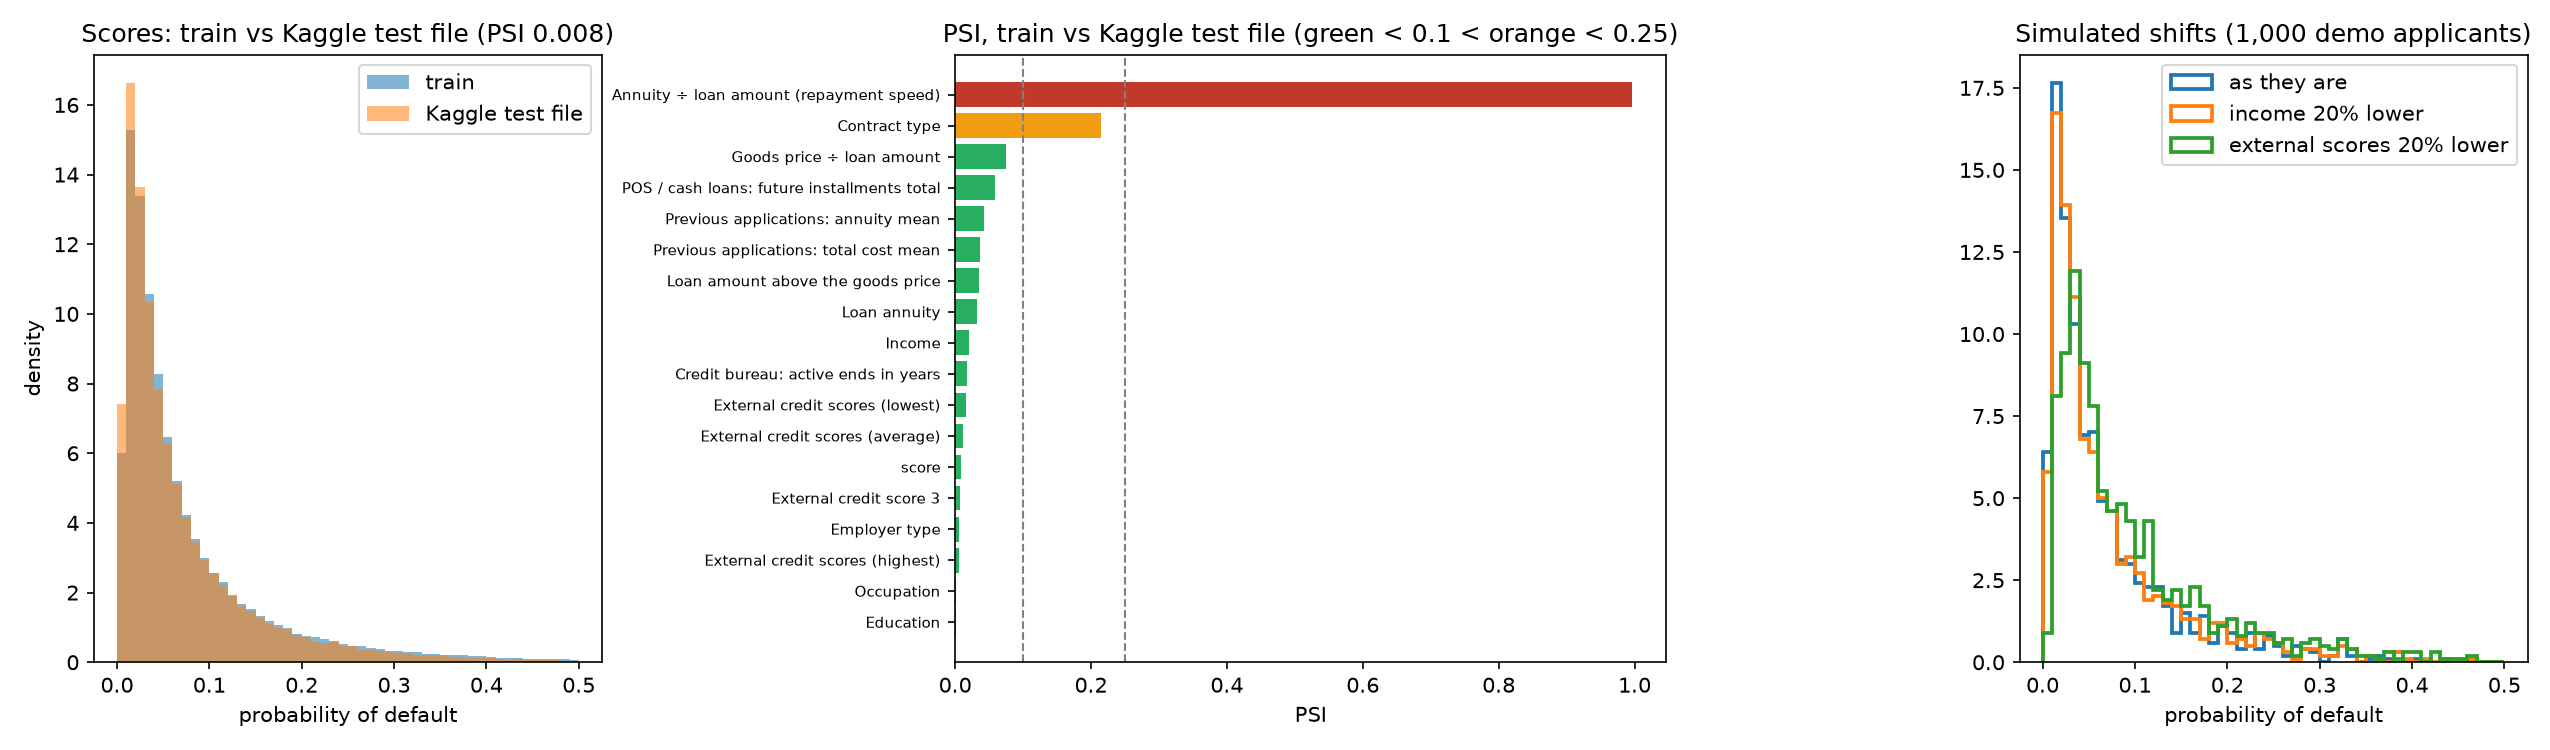
\includegraphics[width=0.9\textwidth]{fig39_drift.png}
\caption{Drift monitoring: scores on train vs the later Kaggle applications (left), PSI of the watched features (middle), and simulated shifts (right).}
\label{fig:drift}
\end{figure*}

% =========================================================================================
\section{Ethics and Limitations}
\label{sec:ethics}
\textbf{Which fairness.} With different base rates, equal error rates and calibration within
groups cannot both hold; we chose equal opportunity for good customers and measured what it
costs. Age is a model input: it is predictive, and older applicants are favoured, but the
approval ratio by age is close to the 80\% rule and the conformal promise does not hold within
age groups. A group-conditional conformal layer would fix this but needs the group when deciding.

\textbf{Reject inference.} Outcomes exist only for loans Home Credit approved in the past, so
the training data is a biased sample of all applicants: people the old policy rejected never
show whether they would have repaid. The model is therefore trustworthy for applicants who look
like past approvals, and its scores for unusual applicants rest on extrapolation.
Semi-supervised reject-inference methods use the unlabelled applicants to correct this, but
without outcomes for rejected people their gains cannot be verified; we state the limitation
rather than claim a correction.

\textbf{Privacy.} The data stays outside the repository; only aggregate tables and figures are
committed. The API validates every input and stores nothing. The public demo contains no real
person and no real model.

\textbf{Inherited bias.} The external scores are the strongest inputs and their origin is
unknown, so any bias in them is inherited.

\textbf{Human in the loop.} The refer zone keeps a person in charge of the 47\% of cases where
the model is unsure, and every automatic decision comes with reasons and a counterfactual, so it
can be contested.

\textbf{Assumptions.} Profit depends on the assumed margin and loss; the conformal guarantee
assumes exchangeability; one lender and one period (data released in 2018). The datasheet and
the model card~\cite{gebru2021,mitchell2019} are in the repository.

% =========================================================================================
\section{Conclusion and Future Work}
A carefully engineered gradient-boosting model reached ROC-AUC 0.790 on untouched test data,
exactly its cross-validation estimate, but the larger contribution is everything around it. Its
probabilities were honest without help; a break-even rule turned them into 13.9\% more profit; a
class-conditional conformal layer kept its error promise on test; every decision comes with
reasons and an actionable counterfactual; and the costs of fairness were measured instead of
assumed.

\textbf{Five lessons.}
(1) Class-imbalance ``fixes'' hurt a model that is already calibrated.
(2) Ranking gains do not always become decision gains.
(3) Fairness interventions move errors between groups and cost calibration.
(4) Structure in the inputs is not structure in the risk.
(5) A promise (conformal) is more useful than a single number, and it costs automation.

\textbf{Future work.} Refit the conformal layer per group where the law allows; evaluate reject
inference with outcome data; and treat credit-limit setting as a sequential decision problem with
reinforcement learning~\cite{sutton2018}, where each limit change affects both repayment and the
data collected next.

\bibliographystyle{IEEEtran}
\bibliography{references}

% =========================================================================================
\clearpage
\onecolumn
\appendices
\section{Glossary}

\begin{table}[!ht]
\centering\small
\caption{Glossary of the terms used in this report, in one line each.}
\begin{tabular}{@{}lp{13.2cm}@{}}
\toprule
Term & Meaning \\
\midrule
Default & The borrower had payment difficulties (\texttt{TARGET} = 1); 8.07\% of applicants. \\
Probability of default ($p$) & The model's output: the estimated chance this applicant defaults. \\
Feature / label & An input number about the applicant / the outcome we try to predict. \\
Train / validation / test split & Data to learn from / to tune the system on / to evaluate once at the end. \\
Cross-validation (CV) & Train on 4 of 5 folds, score the 5th, rotate; every applicant is scored by a model that never saw it. \\
Overfitting & Learning the training data by heart, so new data scores much worse. \\
Leakage & Information from the evaluation data sneaking into training; makes results look too good. \\
ROC-AUC & Chance that a random defaulter gets a higher risk than a random good customer (0.5 random, 1 perfect). \\
Gini, KS & $2\cdot$AUC$-1$; the largest gap between the shares of defaulters and of good customers above a threshold. \\
PR-AUC & Area under the precision--recall curve; focuses on the rare defaulters (random = 0.081). \\
Calibration & Predicted probabilities match observed frequencies (of those given 10\%, about 10\% default). \\
Brier score, ECE & Mean squared error of the probabilities; average gap between predicted and actual rates per bin. \\
Bootstrap CI & Resample the data 1,000 times to see how much a score could vary; the middle 95\% is the interval. \\
Paired bootstrap & The same resamples for two models; a CI for their difference. \\
McNemar test & Compares two models on the cases where exactly one of them is right. \\
Holm correction & Adjusts p-values when several tests are run, so false alarms stay at 5\% overall. \\
Gradient boosting & Many small trees added one by one, each correcting the errors left by the previous ones. \\
Hyperparameter & A setting chosen before training (e.g.\ number of leaves), not learned from the data. \\
SMOTE & Creates synthetic minority examples between real ones; here it hurt. \\
Break-even threshold & Approve if $p < m/(m+\mathrm{LGD})$: where the expected profit of lending turns positive. \\
LGD & Loss given default: the share of the loan lost when a borrower defaults (assumed 50\%). \\
Conformal prediction & Turns a score into a set of possible answers with a guaranteed error rate. \\
Coverage & The share of applicants whose set contains their true outcome (target $1-\alpha$ = 90\%). \\
Exchangeability & New applicants look like (come from the same population as) the calibration applicants. \\
Refer zone & Applicants for whom both answers are possible; a person decides. \\
SHAP value & One feature's push on one prediction; all pushes add up to the prediction. \\
Reason code & A sentence built from the largest risk-raising SHAP values. \\
Counterfactual & The smallest actionable change (here: a smaller loan or a higher income) that changes the decision. \\
LIME & Explains one prediction with a simple local linear model fitted to random perturbations. \\
PDP & The model's average prediction as one feature is varied. \\
Equal opportunity gap & Difference between groups in the share of good customers wrongly declined (our main fairness measure). \\
Disparate impact ratio & Lowest group approval rate divided by the highest; below 0.8 is flagged (``80\% rule''). \\
Proxy & A feature that reveals a protected attribute (gender) even when that attribute is removed. \\
Reweighing & Training weights that make group and outcome look independent. \\
Silhouette & How much closer a point is to its own cluster than to the next one ($-1$ to 1). \\
PSI & Population stability index: how much a distribution has moved (above 0.25 = shift). \\
Drift & New applicants (data drift) or their risk (concept drift) differ from the training period. \\
Reject inference & The problem that outcomes are only known for applicants who were approved in the past. \\
\bottomrule
\end{tabular}
\end{table}

\section{Additional Tables and Figures}

\begin{table}[!ht]
\centering\small
\caption{From-scratch NumPy implementations vs scikit-learn (20,000 training rows, 10,000 check rows).}
\label{tab:scratch}
\footnotesize\setlength{\tabcolsep}{3pt}
\begin{tabular}{@{}lccc@{}}
\toprule
Algorithm & Measure & Scratch & sklearn \\
\midrule
Logistic reg.\ (Newton, MAP) & ROC-AUC & 0.7544 & 0.7544 \\
Bayesian logistic (Laplace) & ROC-AUC & 0.7551 & 0.7544 \\
Gaussian NB & ROC-AUC & 0.6614 & 0.6614 \\
PCA via SVD & var.\ in 30 comp. & 65.7\% & 65.7\% \\
Fisher LDA (30 comp.) & ROC-AUC & 0.7531 & 0.7531 \\
K-means++ ($k=6$) & inertia & 1,466,934 & 1,466,932 \\
GMM with EM ($k=4$) & avg log-lik. & $-20.847$ & $-20.851$ \\
MLP (32 hidden) & ROC-AUC & 0.7053 & 0.7038 \\
\bottomrule
\end{tabular}
\end{table}

\begin{table}[!ht]
\centering\small
\caption{Final LightGBM hyperparameters (Optuna TPE, trial 23).}
\begin{tabular}{@{}ll@{}}
\toprule
Parameter & Value \\
\midrule
learning rate & 0.0219 \\
number of leaves & 17 \\
min.\ rows per leaf & 426 \\
row / feature sampling & 0.951 / 0.272 \\
L2 regularisation & 0.457 \\
trees (refit on all train rows) & 1,871 \\
\bottomrule
\end{tabular}
\end{table}

\begin{table}[!ht]
\centering\small
\caption{Calibration on validation (cross-fitted).}
\begin{tabular}{@{}lccc@{}}
\toprule
 & ROC-AUC & Brier & ECE \\
\midrule
none (raw) & 0.7931 & 0.06529 & 0.0024 \\
Platt (sigmoid) & 0.7930 & 0.06530 & 0.0017 \\
isotonic & 0.7908 & 0.06534 & 0.0012 \\
\bottomrule
\end{tabular}
\end{table}

\begin{table}[!ht]
\centering\small
\caption{Class-imbalance experiment (5-fold CV; actual default rate 0.081).}
\label{tab:imbalance}
\setlength{\tabcolsep}{3pt}
\begin{tabular}{@{}lccc@{}}
\toprule
Variant & ROC-AUC & ECE & mean $p$ \\
\midrule
none & 0.7870 & 0.004 & 0.079 \\
class weights & 0.7852 & 0.254 & 0.335 \\
undersampling (1:2) & 0.7831 & 0.189 & 0.270 \\
imputed control & 0.7858 & 0.004 & 0.079 \\
SMOTE (1:2) & 0.7831 & 0.003 & 0.084 \\
\bottomrule
\end{tabular}
\end{table}

\begin{table}[!ht]
\centering\small
\caption{How to reproduce (from the repository root).}
\begin{tabular}{@{}ll@{}}
\toprule
Command & What it does \\
\midrule
\texttt{make data parquet} & download, convert to Parquet \\
\texttt{make splits features} & frozen splits, 240 features \\
\texttt{notebooks/01--14} & every number in this report \\
\texttt{make test} & 133 unit tests \\
\texttt{make app} / \texttt{make api} & the app / the API \\
\texttt{make mlflow} & the experiment dashboard \\
\texttt{make report} & this PDF \\
\bottomrule
\end{tabular}
\end{table}

\begin{figure}[!ht]
\centering
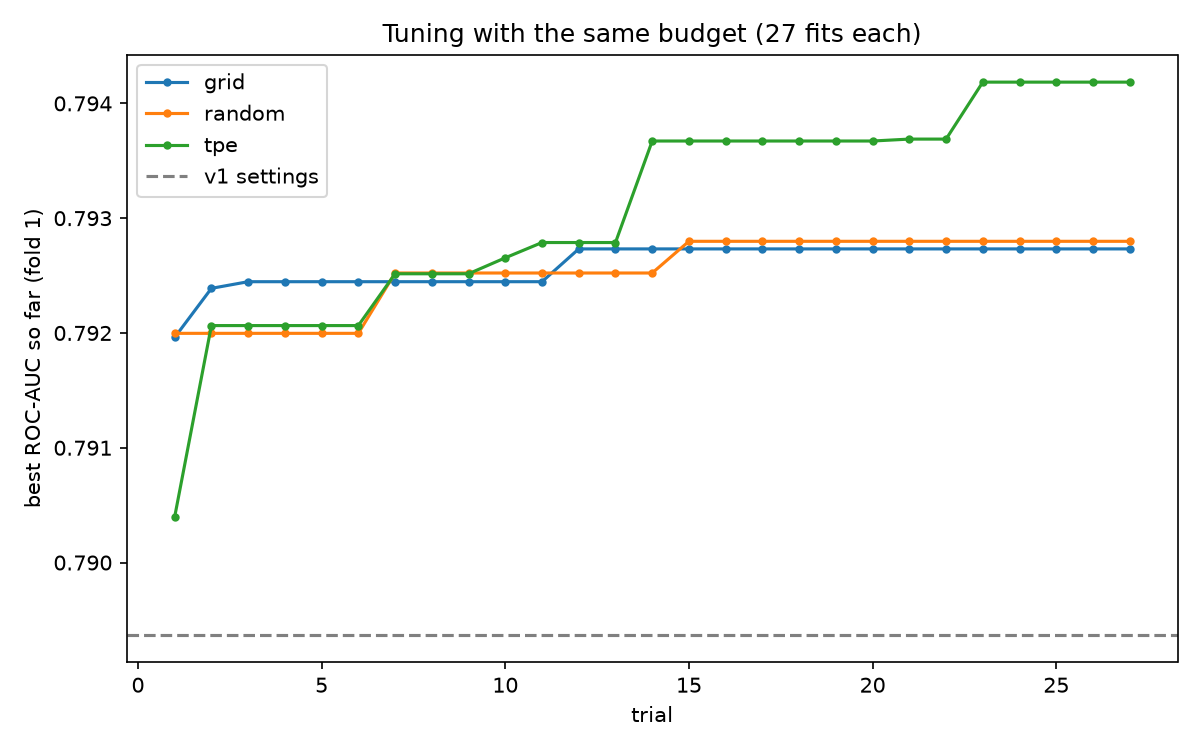
\includegraphics[width=0.6\textwidth]{fig17_tuning_curves.png}
\caption{Best ROC-AUC so far vs number of fits for grid, random and TPE search (fold 1).}
\end{figure}

\begin{figure}[!ht]
\centering
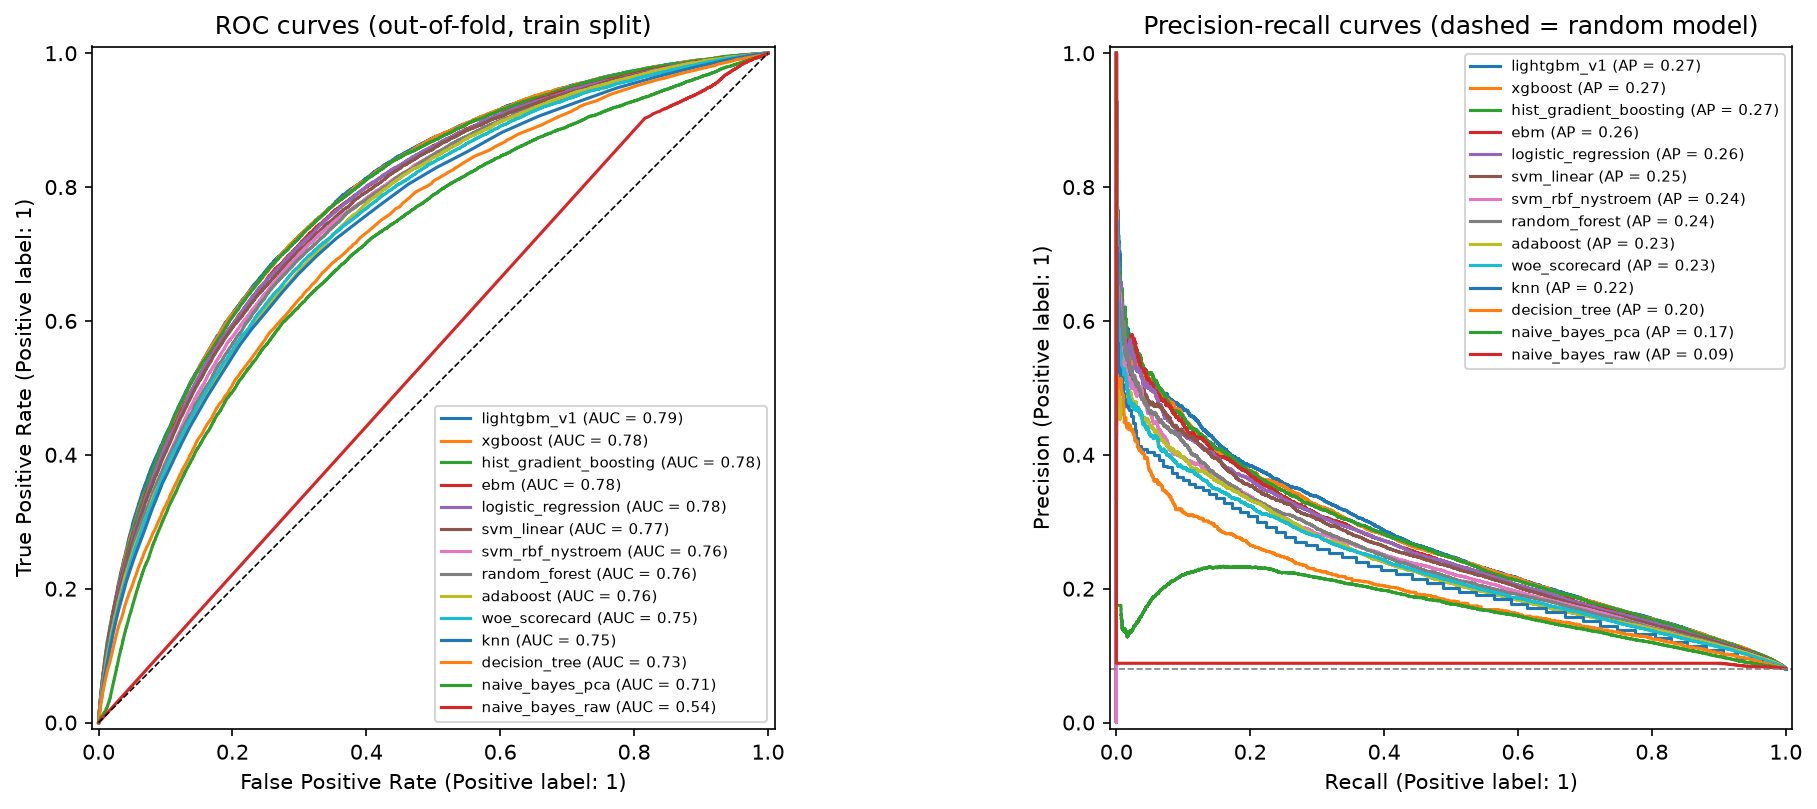
\includegraphics[width=0.85\textwidth]{fig14_ladder_roc_pr.png}
\caption{ROC and precision--recall curves of the model ladder (out-of-fold).}
\end{figure}

\begin{figure}[!ht]
\centering
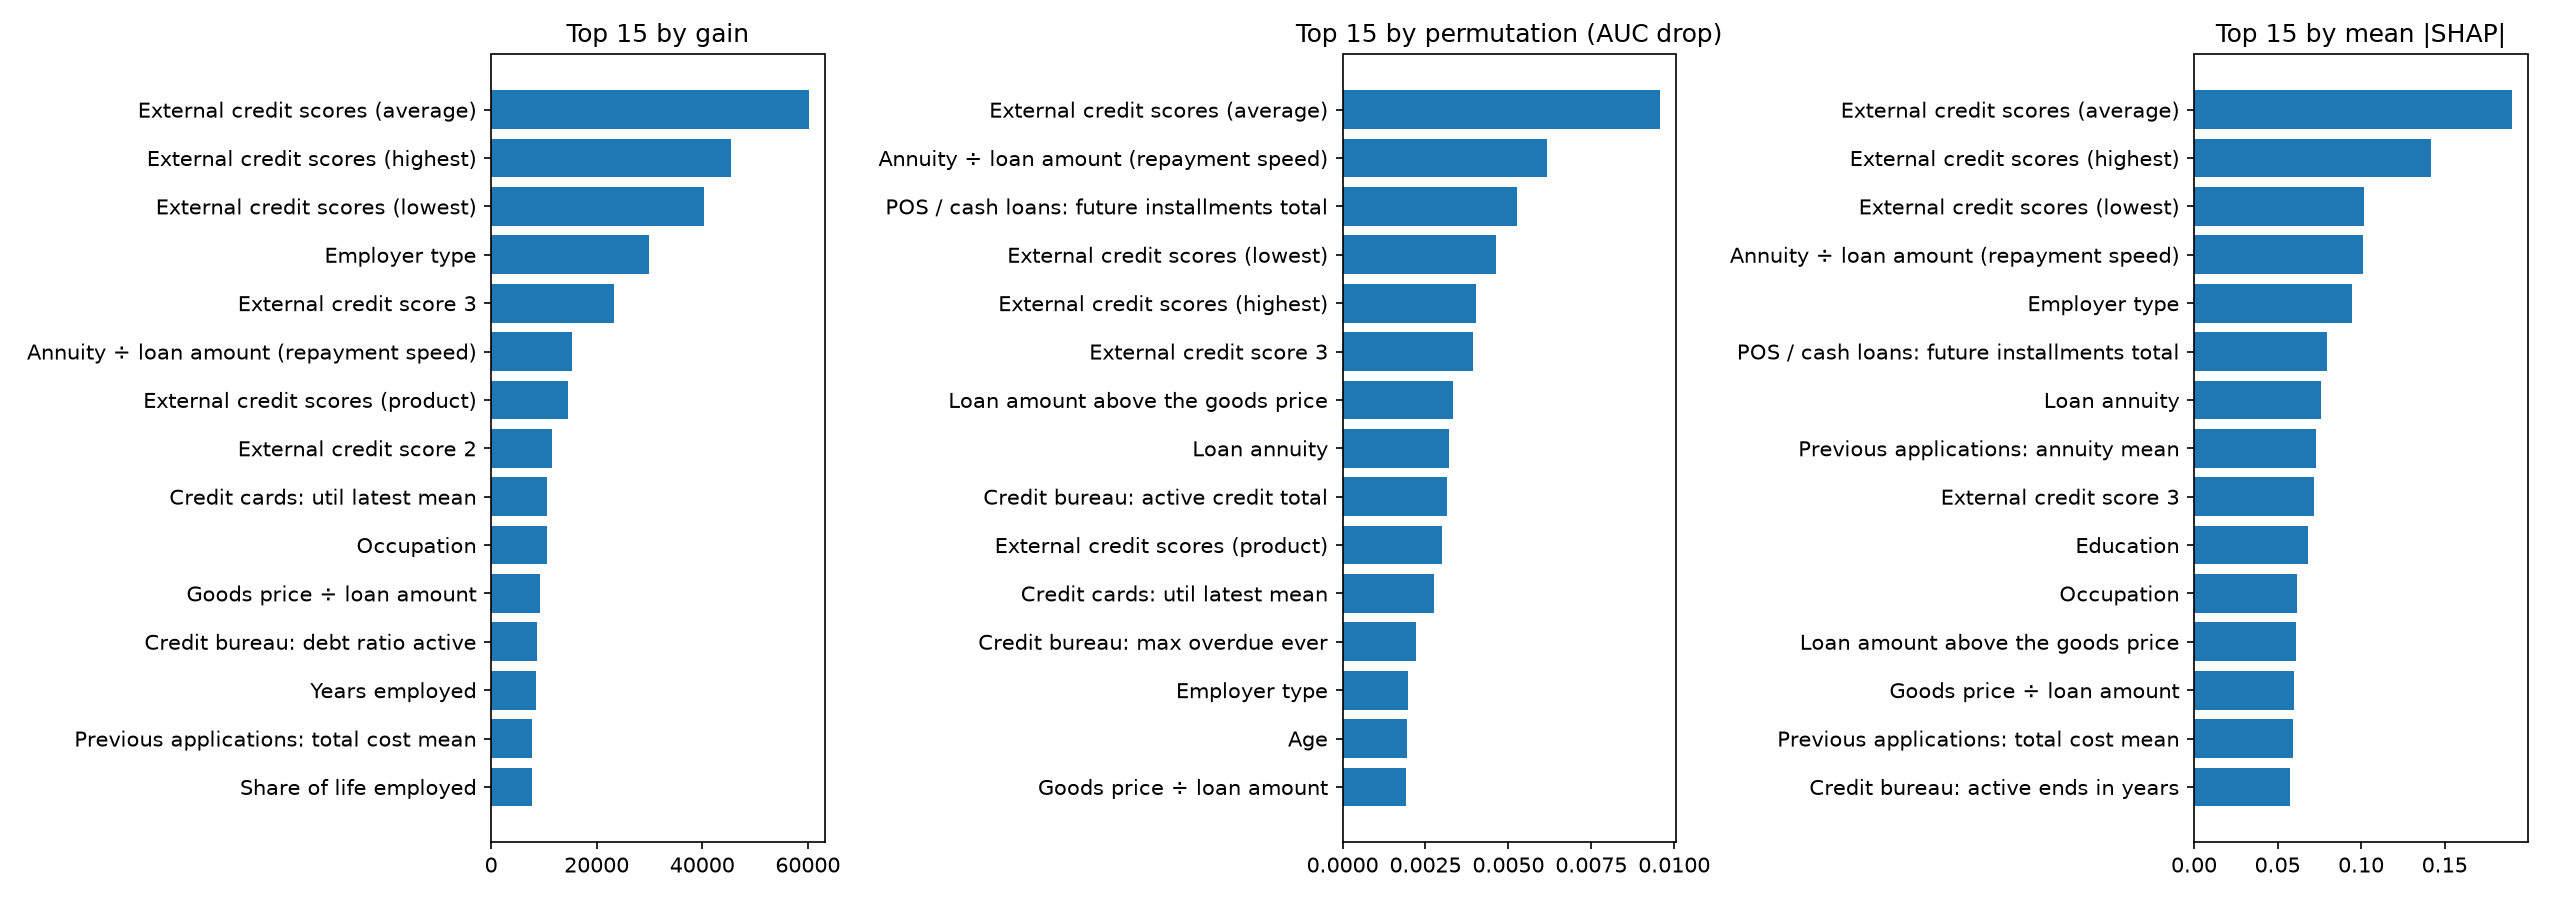
\includegraphics[width=0.85\textwidth]{fig25_importance_methods.png}
\caption{Top features by gain, permutation and mean $|$SHAP$|$.}
\end{figure}

\begin{figure}[!ht]
\centering
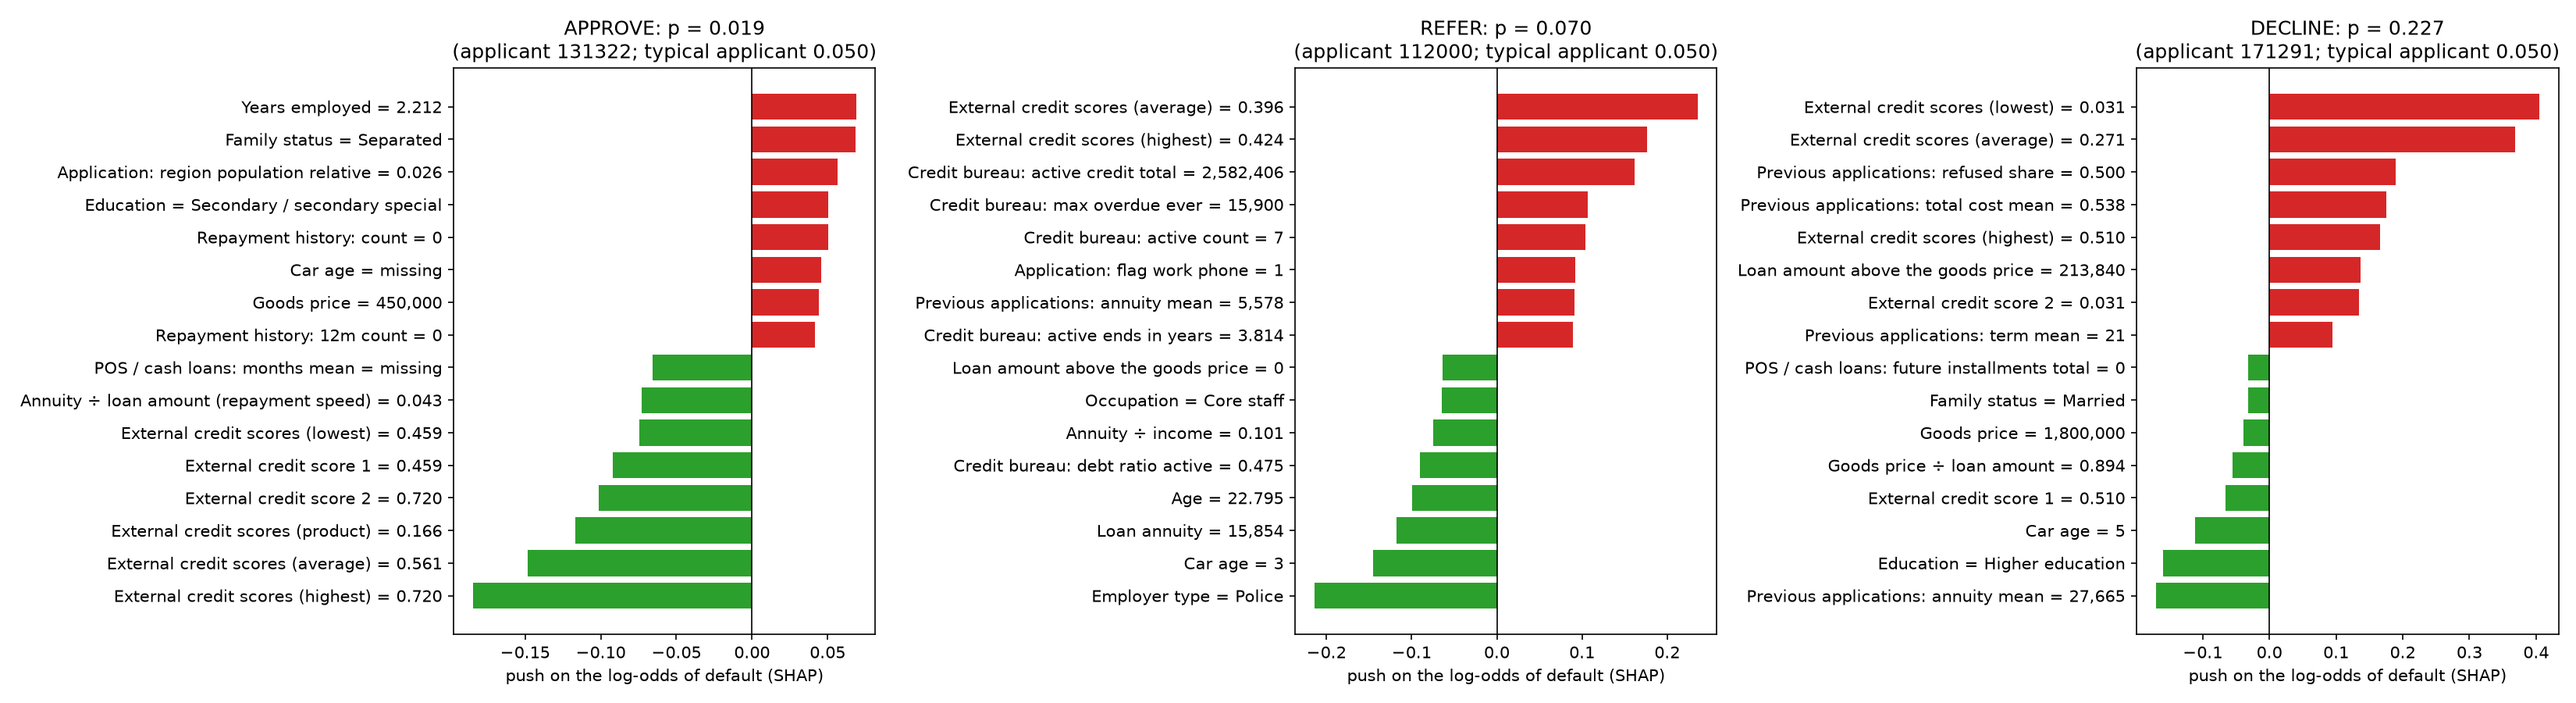
\includegraphics[width=0.85\textwidth]{fig28_local_shap.png}
\caption{Per-applicant SHAP reasons for an approved, a referred and a declined example.}
\end{figure}

\begin{figure}[!ht]
\centering
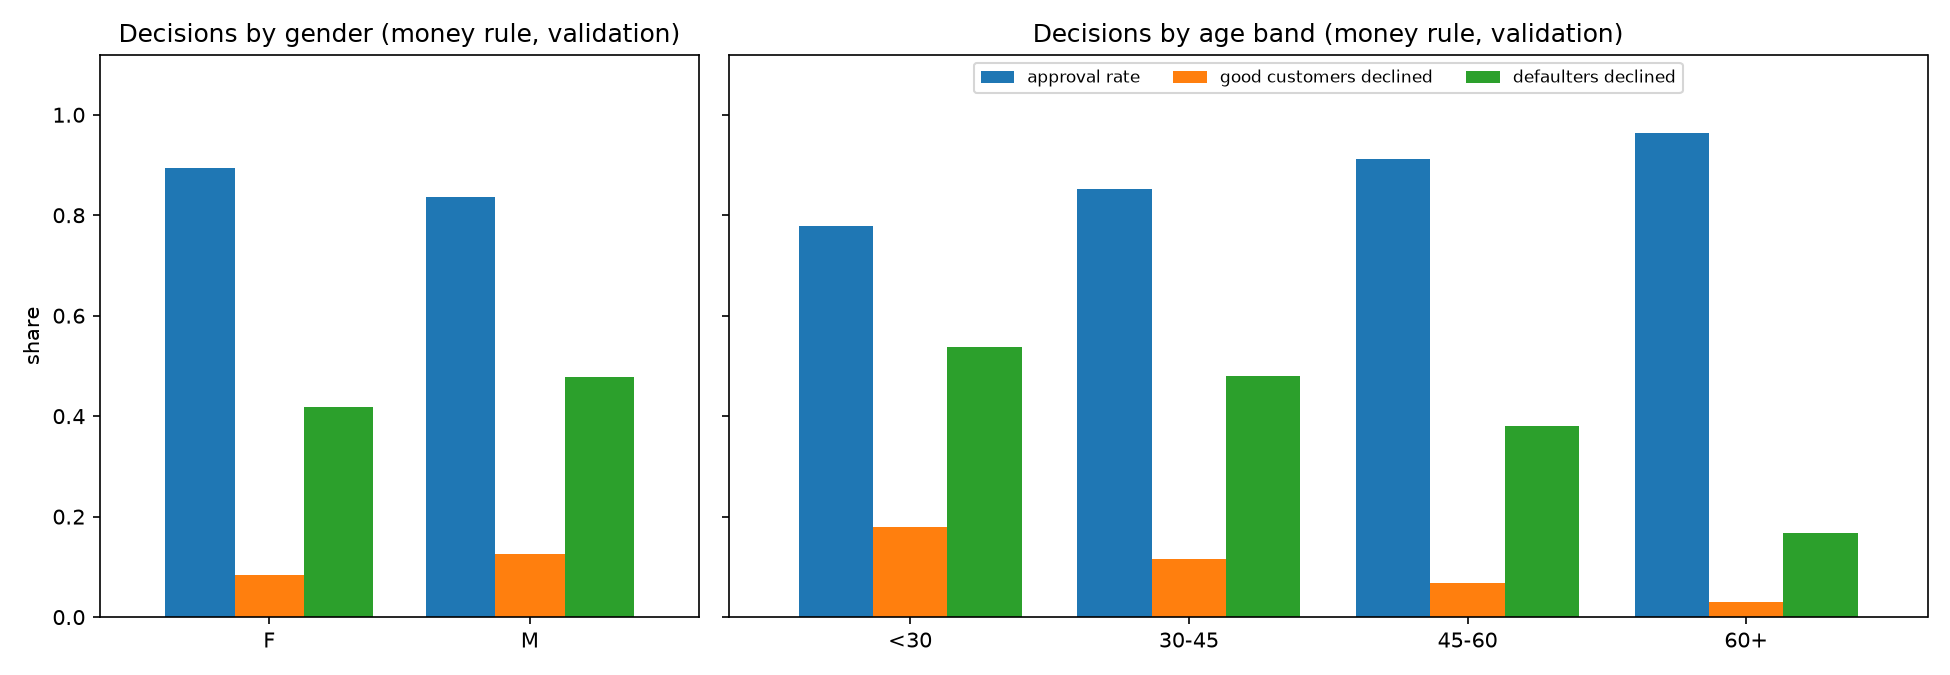
\includegraphics[width=0.85\textwidth]{fig30_fairness_audit.png}
\caption{Decision rates by gender and age band (money rule, validation).}
\end{figure}

\begin{figure}[!ht]
\centering
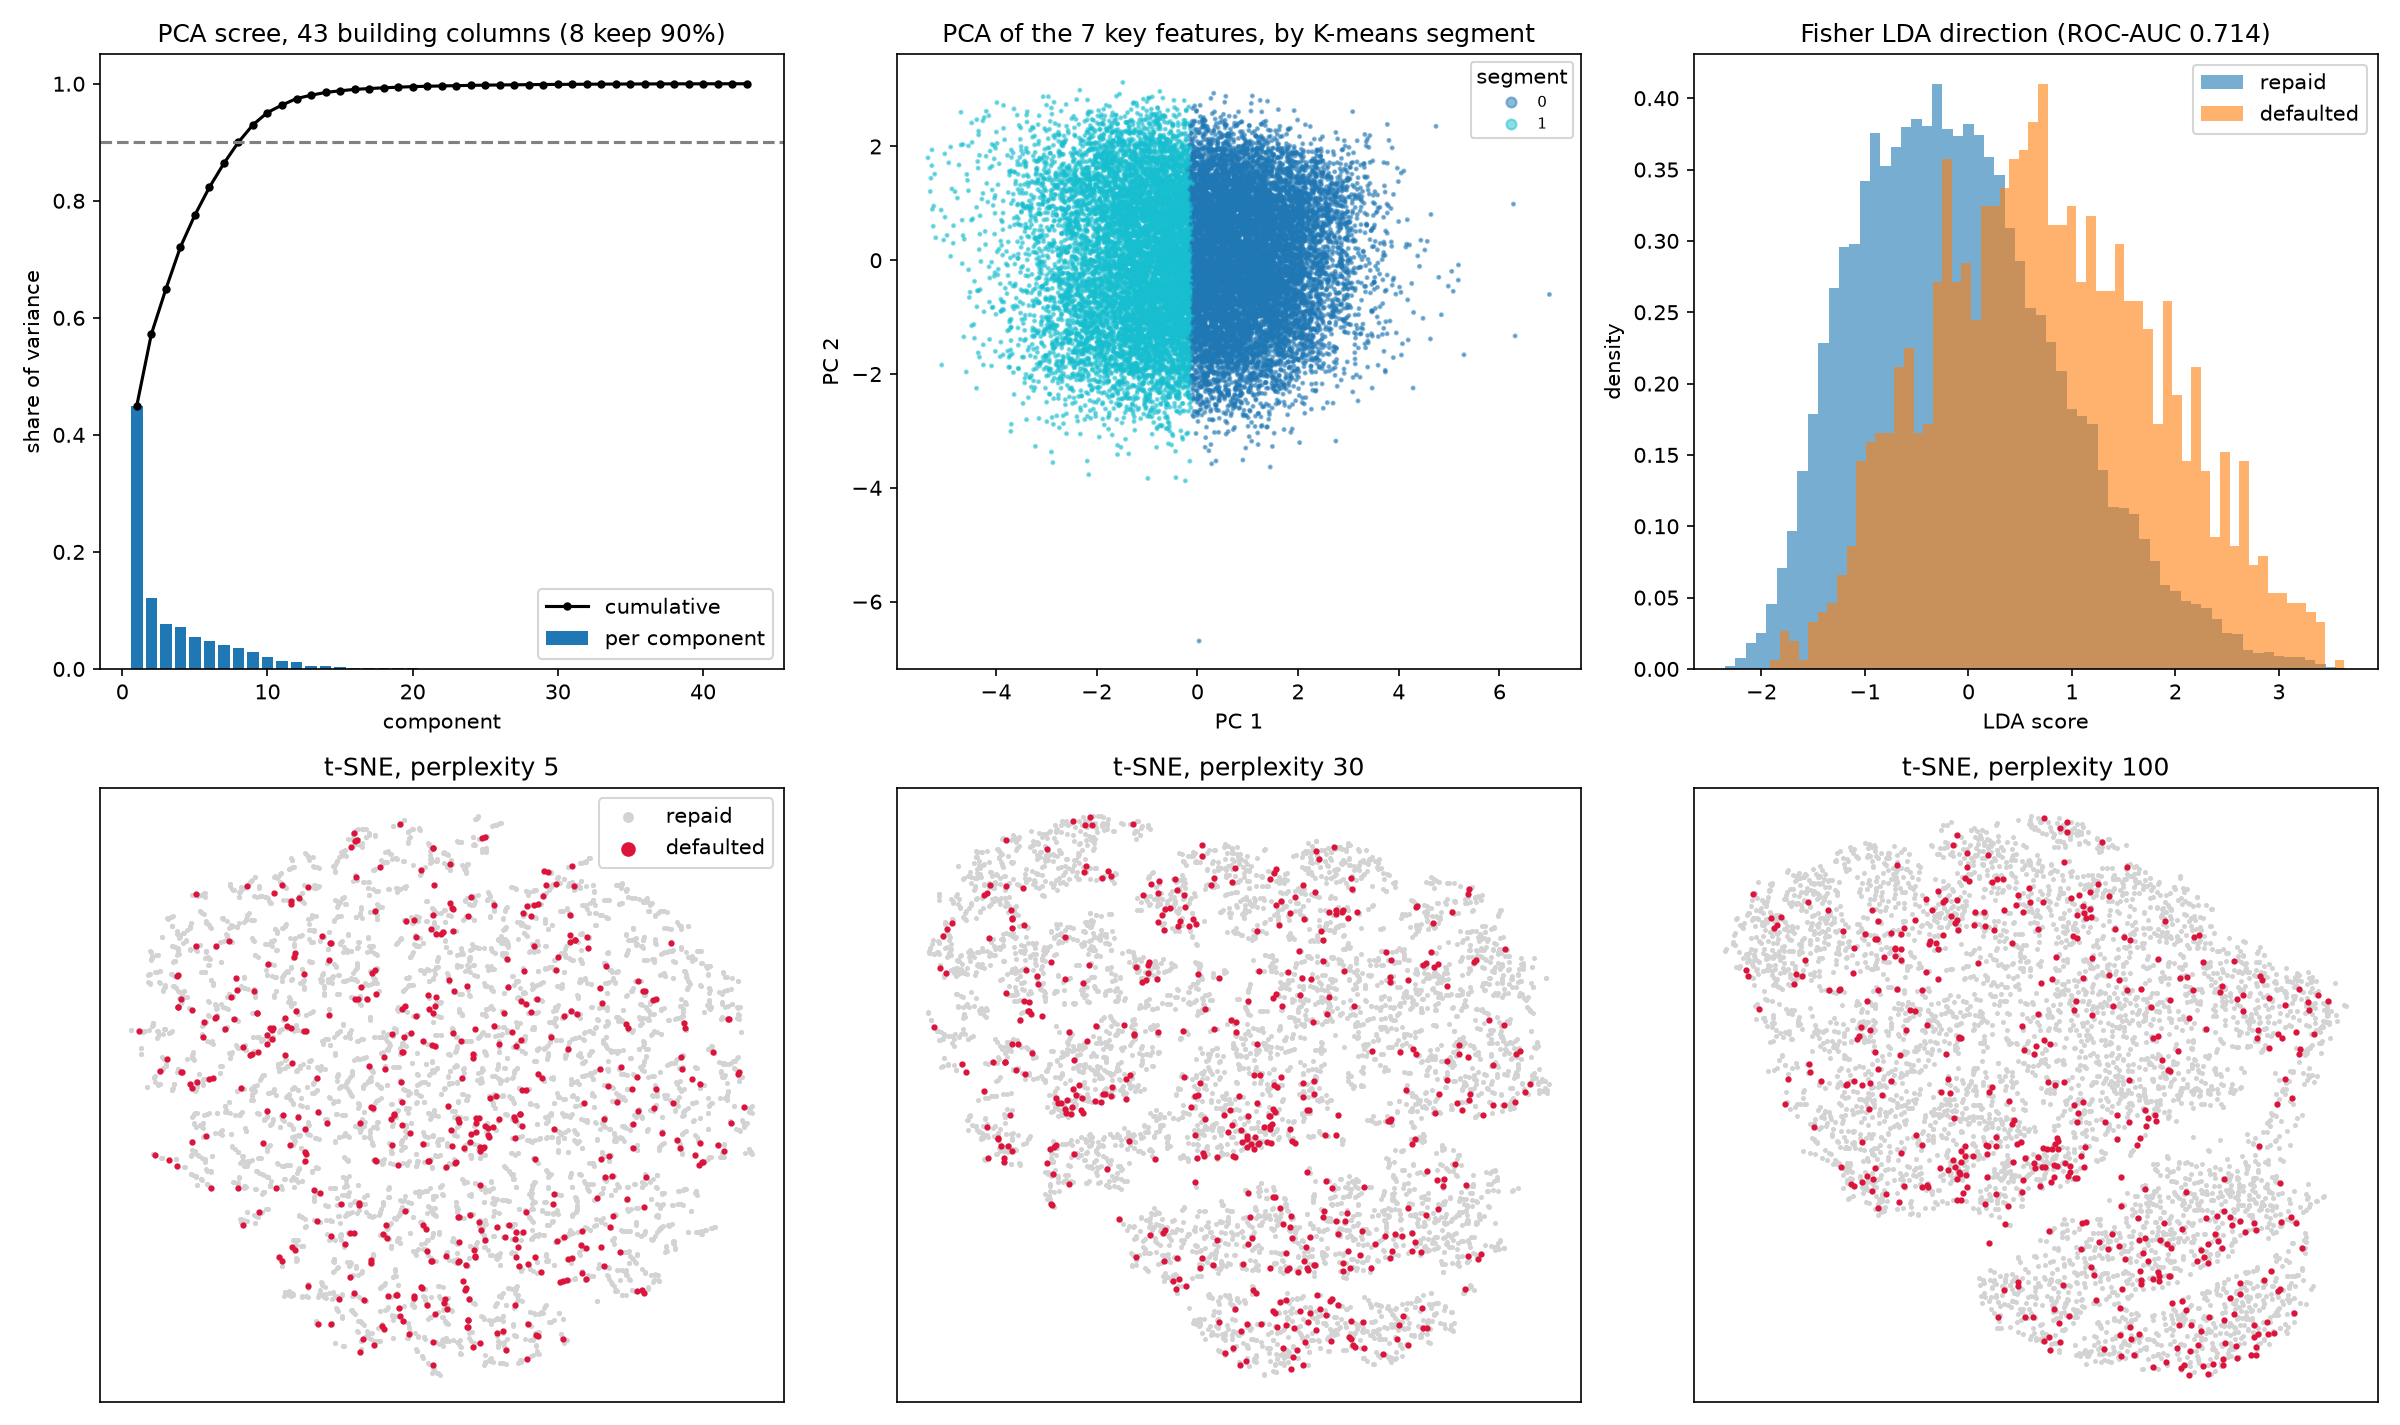
\includegraphics[width=0.85\textwidth]{fig35_maps.png}
\caption{PCA scree of the building columns, PCA of the key features, Fisher LDA projection, and t-SNE at three perplexities.}
\end{figure}

% Screenshots: included automatically once saved under reports/figures/ with these names
\IfFileExists{../figures/mlflow_runs.png}{
\begin{figure}[!ht]
\centering
\includegraphics[width=0.85\textwidth]{mlflow_runs.png}
\caption{MLflow: every cross-validation run of the project, with its metrics.}
\end{figure}}{}
\IfFileExists{../figures/mlflow_compare.png}{
\begin{figure}[!ht]
\centering
\includegraphics[width=0.85\textwidth]{mlflow_compare.png}
\caption{MLflow: comparing the model-ladder runs.}
\end{figure}}{}
\IfFileExists{../figures/mlflow_run.png}{
\begin{figure}[!ht]
\centering
\includegraphics[width=0.85\textwidth]{mlflow_run.png}
\caption{MLflow: the final tuned LightGBM run (parameters and metrics).}
\end{figure}}{}
\IfFileExists{../figures/app_v2_screenshot.png}{
\begin{figure}[!ht]
\centering
\includegraphics[width=0.85\textwidth]{app_v2_screenshot.png}
\caption{The public Streamlit demo (made-up applicants, stand-in model).}
\end{figure}}{}

\end{document}
